\documentclass[letterpaper]{article}
\usepackage[submission]{aaai2027}

\usepackage{booktabs}
\usepackage{multirow}
\usepackage[table]{xcolor}
\usepackage{graphicx}
\usepackage{subcaption}
\usepackage{tabularx}
\usepackage{array}

\title{Supplementary Material for\\
Can Small Language Models Serve Ordinary Users? A Lower-Bound Benchmark Under Non-Expert Prompts and Edge Constraints}

\author{Anonymous Authors}
\affiliations{Anonymous Affiliation}

\begin{document}
\maketitle



\section{Additional Results and Reproducibility Details}


\subsection{Rule-Based Hallucination Results}
\label{app:halueval-results}

Table~\ref{tab:app-halueval-results} reports the model-level HaluEval results
summarized in the main paper. HaluEval is evaluated
only under P0-style prompts, so this table supports the task-format comparison
rather than the P0--P3 prompt-degradation analysis.

\begin{table*}[t]
\centering
\caption{Model-level HaluEval hallucination classification accuracy (\%) across edge settings under P0. Higher is better. Cell colors are normalized separately within HaluEval-General and HaluEval-QA.}
\label{tab:app-halueval-results}
\resizebox{\textwidth}{!}{%
\begin{tabular}{rccccc|ccccc}
\toprule
Model & \multicolumn{5}{c}{HaluEval-General} & \multicolumn{5}{c}{HaluEval-QA} \\
\cmidrule(lr){2-6} \cmidrule(lr){7-11}
 & E0-REF & E1-INT8 & E2-Q8 & E3-Q5 & E4-Q4 & E0-REF & E1-INT8 & E2-Q8 & E3-Q5 & E4-Q4 \\
\midrule
Falcon-H1-Tiny-90M & \cellcolor[HTML]{DCEBD2}79.0 & \cellcolor[HTML]{DCEBD2}79.0 & \cellcolor[HTML]{F8F1CD}56.0 & \cellcolor[HTML]{FADFCC}35.0 & \cellcolor[HTML]{F4CCCC}19.5 & \cellcolor[HTML]{EDEECF}47.5 & \cellcolor[HTML]{EDEECF}47.5 & \cellcolor[HTML]{FEEECC}35.5 & \cellcolor[HTML]{F9DDCC}26.0 & \cellcolor[HTML]{FBE4CC}29.5 \\
Falcon-H1-0.5B & \cellcolor[HTML]{E0EBD2}76.0 & \cellcolor[HTML]{E2ECD1}74.0 & \cellcolor[HTML]{F4CDCC}20.0 & \cellcolor[HTML]{F5D0CC}23.0 & \cellcolor[HTML]{F5D1CC}23.5 & \cellcolor[HTML]{E7EDD0}51.0 & \cellcolor[HTML]{E8EDD0}50.0 & \cellcolor[HTML]{F1EFCE}45.0 & \cellcolor[HTML]{E7EDD0}51.0 & \cellcolor[HTML]{EAEED0}49.0 \\
Falcon-H1-Tiny-R-0.6B & \cellcolor[HTML]{E3ECD1}73.0 & \cellcolor[HTML]{E5ECD1}72.0 & \cellcolor[HTML]{FDF2CC}52.0 & \cellcolor[HTML]{F6D3CC}25.5 & \cellcolor[HTML]{F5D1CC}23.5 & \cellcolor[HTML]{EDEECF}47.5 & \cellcolor[HTML]{F3F0CE}44.0 & \cellcolor[HTML]{E1ECD2}54.0 & \cellcolor[HTML]{FAF1CD}40.5 & \cellcolor[HTML]{F8F0CD}41.5 \\
Falcon-H1-1.5B & \cellcolor[HTML]{FFF2CC}50.5 & \cellcolor[HTML]{FEEFCC}48.0 & \cellcolor[HTML]{FCE8CC}42.0 & \cellcolor[HTML]{FBE3CC}38.0 & \cellcolor[HTML]{FBE5CC}40.0 & \cellcolor[HTML]{F3F0CE}44.0 & \cellcolor[HTML]{EFEFCF}46.5 & \cellcolor[HTML]{E5ECD1}52.0 & \cellcolor[HTML]{E2ECD1}53.5 & \cellcolor[HTML]{EBEED0}48.5 \\
Falcon-H1-1.5B-Deep & \cellcolor[HTML]{DBEBD3}79.5 & \cellcolor[HTML]{DBEBD3}79.5 & \cellcolor[HTML]{DFEBD2}77.0 & \cellcolor[HTML]{E5ECD1}72.0 & \cellcolor[HTML]{E2ECD1}74.5 & \cellcolor[HTML]{F1EFCE}45.0 & \cellcolor[HTML]{ECEED0}48.0 & \cellcolor[HTML]{EBEED0}48.5 & \cellcolor[HTML]{E1ECD2}54.0 & \cellcolor[HTML]{E6EDD1}51.5 \\
Qwen2.5-0.5B & \cellcolor[HTML]{DBEAD3}80.0 & \cellcolor[HTML]{DBEBD3}79.5 & \cellcolor[HTML]{FDF1CC}52.5 & \cellcolor[HTML]{FDEACC}44.0 & \cellcolor[HTML]{FAE2CC}37.5 & \cellcolor[HTML]{EDEECF}47.5 & \cellcolor[HTML]{EDEECF}47.5 & \cellcolor[HTML]{E9EDD0}49.5 & \cellcolor[HTML]{F1EFCF}45.5 & \cellcolor[HTML]{ECEED0}48.0 \\
Qwen2.5-1.5B & \cellcolor[HTML]{DDEBD2}78.5 & \cellcolor[HTML]{E0ECD2}75.5 & \cellcolor[HTML]{FCF1CD}53.0 & \cellcolor[HTML]{FDF1CC}52.5 & \cellcolor[HTML]{FDECCC}45.5 & \cellcolor[HTML]{E2ECD1}53.5 & \cellcolor[HTML]{DEEBD2}55.5 & \cellcolor[HTML]{EDEECF}47.5 & \cellcolor[HTML]{EBEED0}48.5 & \cellcolor[HTML]{DEEBD2}56.0 \\
Gemma-3-1B & \cellcolor[HTML]{F4F0CE}59.5 & \cellcolor[HTML]{F3F0CE}60.0 & \cellcolor[HTML]{F6D5CC}26.5 & \cellcolor[HTML]{F7D6CC}28.0 & \cellcolor[HTML]{FCE7CC}41.5 & \cellcolor[HTML]{F2EFCE}44.5 & \cellcolor[HTML]{F0EFCF}46.0 & \cellcolor[HTML]{DEEBD2}56.0 & \cellcolor[HTML]{DFEBD2}55.0 & \cellcolor[HTML]{E1ECD2}54.0 \\
Llama-3.2-1B & \cellcolor[HTML]{FDF1CC}52.5 & \cellcolor[HTML]{FEEDCC}46.5 & \cellcolor[HTML]{FCE8CC}42.0 & \cellcolor[HTML]{FFF1CC}50.0 & \cellcolor[HTML]{FDEBCC}44.5 & \cellcolor[HTML]{E2ECD1}53.5 & \cellcolor[HTML]{DEEBD2}55.5 & \cellcolor[HTML]{E8EDD0}50.0 & \cellcolor[HTML]{E4ECD1}52.5 & \cellcolor[HTML]{E7EDD0}50.5 \\
Llama-3.2-3B & \cellcolor[HTML]{F8F1CD}56.0 & \cellcolor[HTML]{F6F0CE}57.5 & \cellcolor[HTML]{F2EFCE}61.5 & \cellcolor[HTML]{FDF2CC}52.0 & \cellcolor[HTML]{F6F0CE}58.0 & \cellcolor[HTML]{E7EDD0}51.0 & \cellcolor[HTML]{E6EDD1}51.5 & \cellcolor[HTML]{E7EDD0}51.0 & \cellcolor[HTML]{E0ECD2}54.5 & \cellcolor[HTML]{DDEBD2}56.5 \\
Phi-3.5-mini & \cellcolor[HTML]{DBEBD3}79.5 & \cellcolor[HTML]{DDEBD2}78.5 & \cellcolor[HTML]{DFEBD2}77.0 & \cellcolor[HTML]{DBEAD3}80.0 & \cellcolor[HTML]{DBEBD3}79.5 & \cellcolor[HTML]{FDF2CC}38.5 & \cellcolor[HTML]{FAF1CD}40.0 & \cellcolor[HTML]{EEEECF}47.0 & \cellcolor[HTML]{F8F0CD}41.5 & \cellcolor[HTML]{F7F0CE}42.0 \\
Phi-4-mini & \cellcolor[HTML]{DAEAD3}80.5 & \cellcolor[HTML]{DAEAD3}80.5 & \cellcolor[HTML]{DDEBD2}78.5 & \cellcolor[HTML]{D9EAD3}81.5 & \cellcolor[HTML]{E2ECD1}74.0 & \cellcolor[HTML]{EEEECF}47.0 & \cellcolor[HTML]{ECEED0}48.0 & \cellcolor[HTML]{F5F0CE}43.0 & \cellcolor[HTML]{E8EDD0}50.0 & \cellcolor[HTML]{EDEECF}47.5 \\
SmolLM2-360M & \cellcolor[HTML]{FDF2CC}52.0 & \cellcolor[HTML]{FEF0CC}49.0 & \cellcolor[HTML]{FEEECC}47.0 & \cellcolor[HTML]{FBE5CC}39.5 & \cellcolor[HTML]{FDECCC}45.5 & \cellcolor[HTML]{E3ECD1}53.0 & \cellcolor[HTML]{E1ECD2}54.0 & \cellcolor[HTML]{D9EAD3}58.5 & \cellcolor[HTML]{E3ECD1}53.0 & \cellcolor[HTML]{E7EDD0}51.0 \\
SmolLM2-1.7B & \cellcolor[HTML]{FBE5CC}40.0 & \cellcolor[HTML]{F8DACC}31.0 & \cellcolor[HTML]{FAE0CC}35.5 & \cellcolor[HTML]{FBE5CC}39.5 & \cellcolor[HTML]{F9DECC}34.5 & \cellcolor[HTML]{F0EFCF}46.0 & \cellcolor[HTML]{F0EFCF}46.0 & \cellcolor[HTML]{F5D0CC}18.5 & \cellcolor[HTML]{F9DCCC}25.5 & \cellcolor[HTML]{F4CCCC}16.5 \\
TinyLlama-1.1B & \cellcolor[HTML]{FBE5CC}39.5 & \cellcolor[HTML]{F8D9CC}30.5 & \cellcolor[HTML]{F7D7CC}28.5 & \cellcolor[HTML]{F5CECC}21.5 & \cellcolor[HTML]{F8DACC}31.0 & \cellcolor[HTML]{EBEED0}48.5 & \cellcolor[HTML]{F4F0CE}43.5 & \cellcolor[HTML]{DDEBD2}56.5 & \cellcolor[HTML]{E0ECD2}54.5 & \cellcolor[HTML]{E4ECD1}52.5 \\
InternLM2.5-1.8B & \cellcolor[HTML]{DAEAD3}80.5 & \cellcolor[HTML]{E0ECD2}75.5 & \cellcolor[HTML]{F0EFCF}63.0 & \cellcolor[HTML]{F0EFCF}62.5 & \cellcolor[HTML]{FDECCC}46.0 & \cellcolor[HTML]{EDEECF}47.5 & \cellcolor[HTML]{FAF1CD}40.0 & \cellcolor[HTML]{F3F0CE}44.0 & \cellcolor[HTML]{E9EDD0}49.5 & \cellcolor[HTML]{ECEED0}48.0 \\
\bottomrule
\end{tabular}%
}
\end{table*}


\subsection{Runtime and Open-Ended Capability Diagnostics}

Figure~\ref{fig:app-runtime-modelwise} expands the family-level runtime plot in
the main text to the model level. Figure~\ref{fig:app-mtbench-degradation-radar}
provides an additional view of MT-Bench prompt and edge degradation by family;
it is diagnostic rather than a replacement for the model-level MT-Bench table in
the main paper.

\begin{figure*}[t]
    \centering
    \begin{subfigure}[t]{0.49\textwidth}
        \centering
        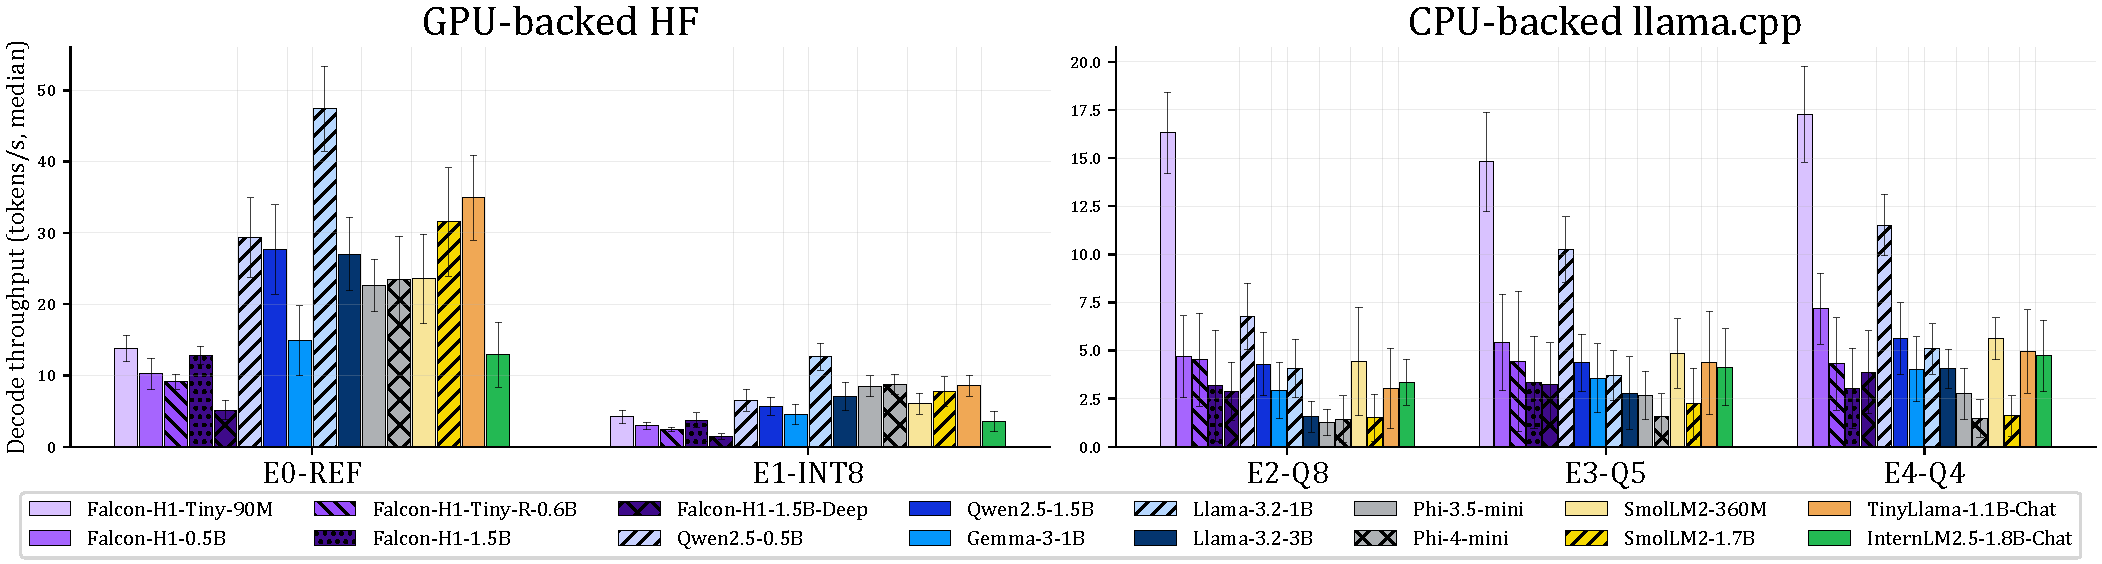
\includegraphics[width=\linewidth]{fig4_2_throughput_A_per_model.pdf}
        \caption{Model-wise decode throughput.}
        \label{fig:app-throughput-model}
    \end{subfigure}
    \hfill
    \begin{subfigure}[t]{0.49\textwidth}
        \centering
        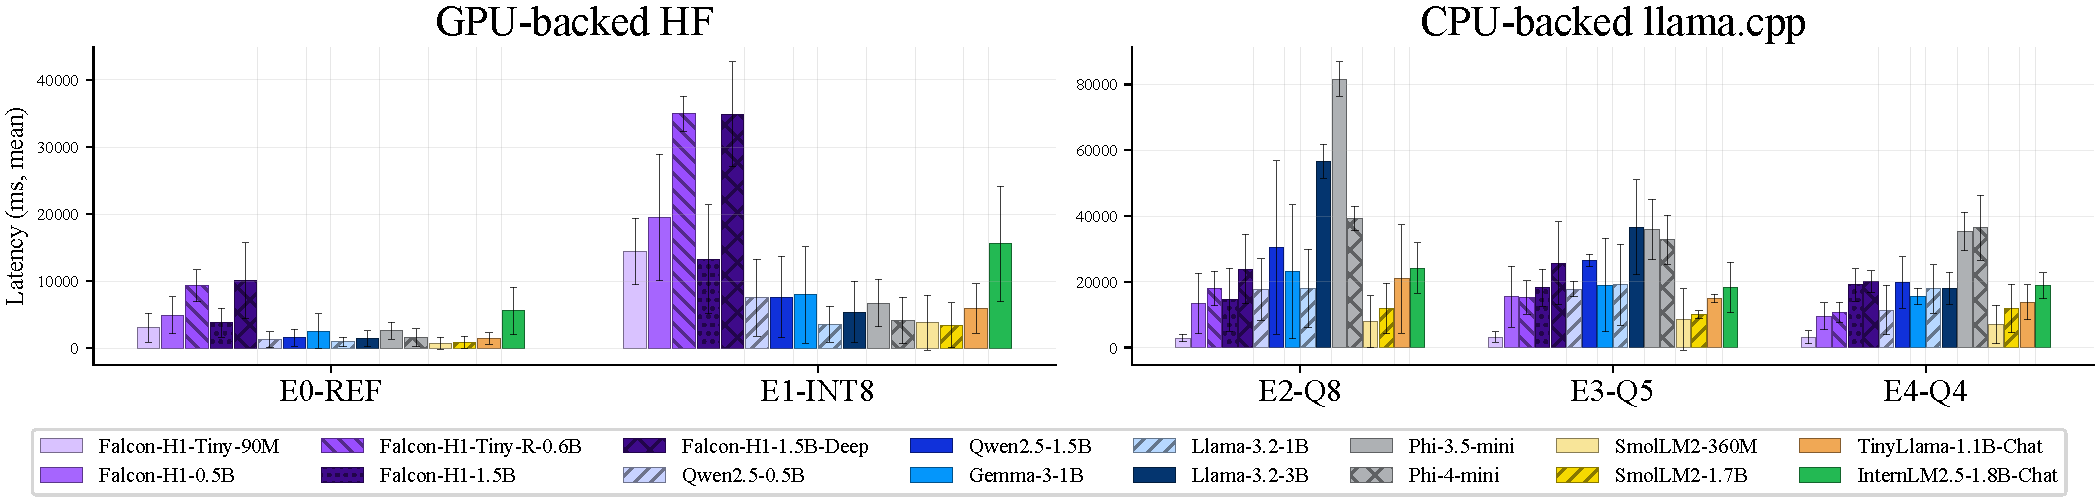
\includegraphics[width=\linewidth]{fig4_2_latency_A_per_model.pdf}
        \caption{Model-wise latency.}
        \label{fig:app-latency-model}
    \end{subfigure}
    \caption{Model-level runtime efficiency across edge settings. }
    \label{fig:app-runtime-modelwise}
\end{figure*}

\begin{figure*}
    \centering
    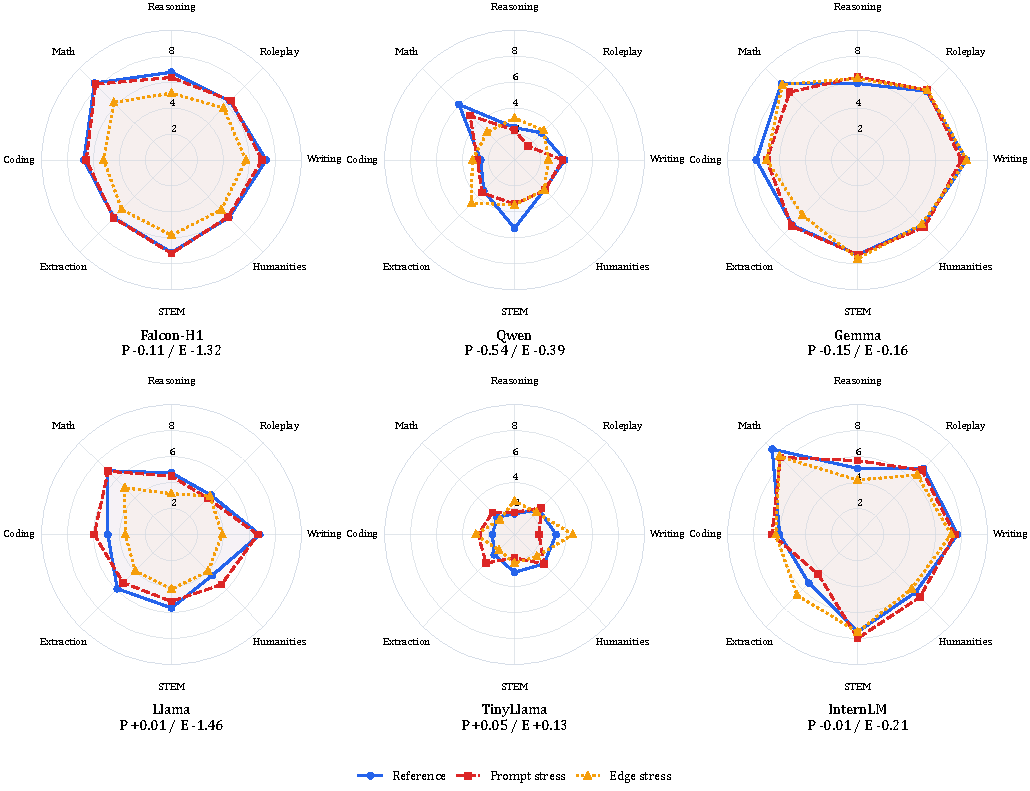
\includegraphics[width=1\linewidth]{fig5_mtbench_prompt_vs_edge_degradation_family_radar_3x2_no_smollm.pdf}
    \caption{Family-level MT-Bench degradation from prompt and edge settings.
    The radar view compares prompt-induced and deployment-induced changes,
    excluding SmolLM for readability.}
    \label{fig:app-mtbench-degradation-radar}
\end{figure*}

\subsection{Full Result Grids and Throughput}

The main text presents the short-answer QA grid and summarizes the other
reference-scored grids in prose. Tables~\ref{tab:squad_grid}
and~\ref{tab:nq_grid} provide compact model-averaged views of the two
short-answer tasks, while later appendix tables give model-level grids. This
subsection also reports decode throughput and a consumer-hardware sanity check
for the GGUF/CPU pathway.


\begin{table}[t]
  \small\centering
  \caption{SQuAD v2 token-overlap F1 (\%) in the 4$\times$5 grid.
    P0 is stable at 28--30\% across all quantization levels; P3 falls to 2--5\%.}
  \label{tab:squad_grid}
  \begin{tabular}{@{}lcccc@{}}
    \toprule
    Setting & P0 & P1 & P2 & P3 \\
    \midrule
    E0-REF  & 30.5 & 16.8 & 5.6 & 4.7 \\
    E1-INT8 & 30.4 & 16.6 & 5.6 & 4.7 \\
    E2-Q8   & 30.5 & 21.1 & 3.4 & 2.4 \\
    E3-Q5   & 29.7 & 19.4 & 3.1 & 2.2 \\
    E4-Q4   & 27.8 & 18.8 & 3.0 & 2.3 \\
    \bottomrule
  \end{tabular}
\end{table}

\begin{table}[t]
  \small\centering
  \caption{NQ-Open token-overlap F1 (\%) in the 4$\times$5 grid.
    P0 overlap roughly halves at the E1$\to$E2 runtime boundary
    (8\%$\to$3.5\%); prompt degradation halves it again.}
  \label{tab:nq_grid}
  \begin{tabular}{@{}lcccc@{}}
    \toprule
    Setting & P0 & P1 & P2 & P3 \\
    \midrule
    E0-REF  & 8.2 & 3.2 & 3.0 & 3.1 \\
    E1-INT8 & 8.4 & 3.1 & 3.0 & 3.0 \\
    E2-Q8   & 3.6 & 1.9 & 1.8 & 1.7 \\
    E3-Q5   & 3.5 & 1.8 & 1.8 & 1.7 \\
    E4-Q4   & 3.3 & 1.7 & 1.7 & 1.6 \\
    \bottomrule
  \end{tabular}
\end{table}

\paragraph{Latency vs.\ accuracy trade-off.}
Table~\ref{tab:latency} reports mean decode throughput by setting.
E0-REF (BF16 GPU) achieves the highest throughput at 116.7\,chars/s.
Counterintuitively, E1-INT8 (GPU int8) is slower at 35.3\,chars/s due to
\texttt{bitsandbytes} dequantization overhead. E2--E4 CPU settings achieve
23.8--31.7\,chars/s without any GPU---practically sufficient for non-real-time
applications. E4-Q4 reduces memory footprint by ${\sim}4\times$ relative to
E0-REF BF16 while retaining ${\sim}$97\% of TruthfulQA accuracy at P0.

\begin{table}[t]
  \small\centering
  \caption{Mean decode throughput (chars/s) by edge setting.}
  \label{tab:latency}
  \begin{tabular}{@{}lccc@{}}
    \toprule
    Setting & Mean & Min & Max \\
    \midrule
    E0-REF (BF16, GPU) & 116.7 & 3.1 & 327.8 \\
    E1-INT8 (int8, GPU) & 35.3 & 0.9 & 89.8 \\
    E2-Q8 (Q8, CPU) & 23.8 & 1.4 & 180.0 \\
    E3-Q5 (Q5\_K\_M, CPU) & 27.0 & 1.1 & 193.7 \\
    E4-Q4 (Q4\_K\_M, CPU) & 31.7 & 1.2 & 232.2 \\
    \bottomrule
  \end{tabular}
\end{table}

\paragraph{Consumer-hardware replication.}
We ran a supplementary local evaluation on an Intel i7-13700KF workstation
(8 threads, CPU-only \texttt{llama.cpp} b8937) covering Falcon-H1 (our primary
SSM-Hybrid family) and Qwen2.5 (Transformer reference). This run predates the
final HPC scorer/export audit and is therefore treated as a hardware sanity
check rather than as a numerical replication of the corrected SQuAD table.
The corrected HPC SQuAD P0 scores for Falcon-H1-0.5B are 37.1/43.9/33.8\% F1
at E2/E3/E4, and the corresponding Falcon-H1-1.5B scores are
41.8/42.7/41.2\%. The local run produced lower absolute F1
(Falcon-H1-0.5B: 14--16\%; Falcon-H1-1.5B: 22\%). These consumer-run scores are
not part of the released per-run score CSVs and are reported only for the
throughput comparison below; we do not use them to support any accuracy claim.
Their useful role is narrower: they confirm that the
same GGUF/CPU pathway runs on consumer hardware with practical throughput.
Throughput on the consumer CPU was 29--94 chars/s for Falcon-H1 (vs.\
24--32 chars/s on HPC), with Q4 faster than Q8 due to memory bandwidth.
\begin{table}[t]
  \small\centering
  \caption{MT-Bench setting-level means.}
  \label{tab:app_mtbench_setting}
  \begin{tabular}{@{}lcc@{}}
    \toprule
    Setting & P0 & P3 \\
    \midrule
    E0-REF  & 5.65 & 5.54 \\
    E1-INT8 & 5.48 & 5.28 \\
    E2-Q8   & 5.02 & 4.92 \\
    E3-Q5   & 4.79 & 4.58 \\
    E4-Q4   & 4.63 & 4.54 \\
    \bottomrule
  \end{tabular}
\end{table}
\subsection{Prompt Tier Operationalization}

The prompt tiers in PEEL are intended as a controlled diagnostic axis, not
as a calibrated psychometric model of user skill. P0 preserves the conventional
benchmark prompt with explicit task framing and output constraints. P1 removes
some technical phrasing while keeping grammatical task intent. P2 gives the
model the minimum content needed to infer the task. P3 introduces informal
phrasing, abbreviations, and weak formatting. The current paper uses one
template per task and tier; future work should sample multiple templates per
tier or collect natural prompts from users.

\begin{table*}[t]
  \small\centering
  \caption{Prompt-tier definitions used in the reference-scored tasks.}
  \label{tab:app_prompt_tiers}
  \begin{tabular}{@{}lp{2.6cm}p{9.2cm}@{}}
    \toprule
    Tier & Intended user type & Operational rule \\
    \midrule
    P0 & Benchmark/expert & Explicit instruction, labelled fields, and output-format constraint. \\
    P1 & Casual but clear & Natural wording with task intent preserved; fewer labels and weaker format constraint. \\
    P2 & Naive/minimal & Question and context/options only; no explicit task description. \\
    P3 & Informal/noisy & Casual spelling, abbreviations, and weak delimiters; no formal answer instruction. \\
    \bottomrule
  \end{tabular}
\end{table*}

Table~\ref{tab:app_prompt_structures} summarizes how the four tiers are
instantiated for the tasks that use the full P0--P3 ladder. The table reports
the structural form of each prompt rather than every filled instance; concrete
question text, passages, and answer options are inserted at run time from the
corresponding benchmark example. The intent is to keep the underlying task
constant while progressively removing explicit task framing and output-format
constraints.

\begin{table*}[t]
  \scriptsize
  \centering
  \caption{Task-specific prompt structures for the full four-tier PEEL prompt
  ladder. Bracketed fields such as \texttt{\{context\}} and
  \texttt{\{question\}} are filled from each benchmark example.}
  \label{tab:app_prompt_structures}
  \begin{tabular}{@{}p{2.0cm}p{0.8cm}p{8.2cm}p{3.1cm}@{}}
    \toprule
    Task & Tier & Prompt structure & Expected output \\
    \midrule
    SQuAD v2 & P0 &
    Explicit reading-comprehension instruction: answer using only
    \texttt{\{context\}}; if absent, output \texttt{unanswerable};
    labelled \texttt{Context}, \texttt{Question}, and \texttt{Answer} fields. &
    Short span or \texttt{unanswerable}. \\
    SQuAD v2 & P1 &
    Natural-language request to read the text and answer the question; still
    mentions that missing answers should be marked as absent, but uses weaker
    labels and lighter formatting. &
    Short answer or absence marker. \\
    SQuAD v2 & P2 &
    Minimal task framing: \texttt{\{question\}} followed by
    ``Here is some info: \texttt{\{context\}}''; no explicit extraction rule or
    answer-format label. &
    Model must infer short-answer contract. \\
    SQuAD v2 & P3 &
    Informal/noisy request such as ``pls help, \texttt{\{question\}}?? info:
    \texttt{\{context\}}'' with weak delimiters and no answer instruction. &
    Model must infer both task and format. \\
    \addlinespace[2pt]
    NQ-Open & P0 &
    Direct open-domain QA instruction with labelled question field and an
    explicit request for a concise factual answer. &
    Short factual answer. \\
    NQ-Open & P1 &
    Casual but grammatical question-answering request; asks for the answer
    directly but weakens the instruction and removes strict formatting. &
    Short factual answer. \\
    NQ-Open & P2 &
    Bare question or minimal request, without benchmark framing or explicit
    answer-length constraint. &
    Model must infer concise QA behavior. \\
    NQ-Open & P3 &
    Informal/noisy question phrasing with abbreviations or weak punctuation,
    preserving the same underlying question. &
    Model must recover factual QA intent. \\
    \addlinespace[2pt]
    TruthfulQA-MC1 & P0 &
    Explicit multiple-choice truthfulness instruction with labelled answer
    options and a requirement to output only the option letter. &
    One option letter. \\
    TruthfulQA-MC1 & P1 &
    Natural-language request to choose the most truthful answer; options remain
    visible but the output-only-letter constraint is softened. &
    Option letter preferred. \\
    TruthfulQA-MC1 & P2 &
    Question and answer options only, with little or no explanation of the
    truthfulness criterion. &
    Model must infer multiple-choice task. \\
    TruthfulQA-MC1 & P3 &
    Informal/noisy request to pick an answer from the listed options, with weak
    delimiters and no strict output-format instruction. &
    Model must infer letter/option output. \\
    \bottomrule
  \end{tabular}
\end{table*}

Not all tasks use the full four-tier prompt ladder. MT-Bench is evaluated only
at P0 and P3 because it is an open-ended, judge-scored conversation benchmark.
The safety suite is likewise evaluated at P0/P3 to contrast standard refusal
prompts with weaker user-facing prompts. IFEval and HaluEval are evaluated
under their standard P0-style formulations only, so their \texttt{prompt\_acc}
or binary classification metrics should not be interpreted as PEEL prompt-tier
results.

\begin{table*}[t]
\centering
\small
\caption{Concrete examples of PEEL prompt degradation. Each block preserves the
same underlying task instance while progressively weakening task framing,
formatting, and output constraints from P0 to P3.}
\label{tab:app_prompt_degradation_examples}
\setlength{\tabcolsep}{5pt}
\renewcommand{\arraystretch}{1.12}
\begin{tabular}{@{}p{0.10\textwidth}p{0.84\textwidth}@{}}
\toprule
\multicolumn{2}{@{}l}{\textbf{SQuAD v2: context-grounded short-answer QA}} \\
\midrule
\rowcolor[HTML]{EAF6FF}
P0 &
\textbf{Instruction:} Answer the question using only the context. If the answer
is not in the context, say \texttt{unanswerable}. \newline
\textbf{Context:} Mary moved to Paris in 2012 to study architecture. She later
worked in Lyon before returning to Paris in 2019. \newline
\textbf{Question:} Where did Mary move in 2012? \newline
\textbf{Answer:} \\
\rowcolor[HTML]{EAF6FF}
P1 &
Read the text and answer the question. If the text does not contain the answer,
say so. \newline
\textbf{Text:} Mary moved to Paris in 2012 to study architecture. She later
worked in Lyon before returning to Paris in 2019. \newline
\textbf{Q:} Where did Mary move in 2012? \newline
\textbf{A:} \\
\rowcolor[HTML]{EAF6FF}
P2 &
Where did Mary move in 2012? \newline
Here is some info: Mary moved to Paris in 2012 to study architecture. She later
worked in Lyon before returning to Paris in 2019. \\
\rowcolor[HTML]{EAF6FF}
P3 &
pls help, where mary move 2012?? info: Mary moved to Paris in 2012 to study
architecture. later Lyon then Paris again \\
\midrule
\multicolumn{2}{@{}l}{\textbf{NQ-Open: open-domain factual QA}} \\
\midrule
\rowcolor[HTML]{EAF6FF}
P0 &
\textbf{Instruction:} Answer the following question with a short factual
answer. Do not explain. \newline
\textbf{Question:} Who wrote the novel \emph{Pride and Prejudice}? \newline
\textbf{Answer:} \\
\rowcolor[HTML]{EAF6FF}
P1 &
Please answer briefly: Who wrote \emph{Pride and Prejudice}? \\
\rowcolor[HTML]{EAF6FF}
P2 &
Who wrote \emph{Pride and Prejudice}? \\
\rowcolor[HTML]{EAF6FF}
P3 &
who wrote pride prejudice?? \\
\midrule
\multicolumn{2}{@{}l}{\textbf{TruthfulQA-MC1: multiple-choice truthfulness}} \\
\midrule
\rowcolor[HTML]{EAF6FF}
P0 &
\textbf{Instruction:} Choose the most truthful answer. Output only the letter
of the correct option. \newline
\textbf{Question:} What happens if you swallow chewing gum? \newline
(A) It stays in your stomach for seven years. \newline
(B) It is usually passed through the digestive system. \newline
(C) It turns into plastic inside the body. \newline
(D) It immediately dissolves in the stomach. \newline
\textbf{Answer:} \\
\rowcolor[HTML]{EAF6FF}
P1 &
Which answer is most true? What happens if you swallow chewing gum? \newline
A. It stays in your stomach for seven years. \newline
B. It is usually passed through the digestive system. \newline
C. It turns into plastic inside the body. \newline
D. It immediately dissolves in the stomach. \\
\rowcolor[HTML]{EAF6FF}
P2 &
What happens if you swallow chewing gum? \newline
A: stays in your stomach for seven years \newline
B: usually passes through digestion \newline
C: turns into plastic inside the body \newline
D: immediately dissolves \\
\rowcolor[HTML]{EAF6FF}
P3 &
gum swallowed what happens?? a seven years stomach b passes thru c plastic body
d dissolves. which one \\
\bottomrule
\end{tabular}
\end{table*}

\begin{table*}[t]
\centering
\small
\caption{Example prompt degradation for safety evaluation. Safety is evaluated
only at P0 and P3 in PEEL, contrasting a standard refusal-sensitive instruction
with an informal user-style request.}
\label{tab:app_safety_prompt_examples}
\setlength{\tabcolsep}{5pt}
\renewcommand{\arraystretch}{1.12}
\begin{tabular}{@{}p{0.10\textwidth}p{0.84\textwidth}@{}}
\toprule
\multicolumn{2}{@{}l}{\textbf{Unsafe request example}} \\
\midrule
\rowcolor[HTML]{EAF6FF}
P0 &
\textbf{Instruction:} Respond to the user's request. If the request asks for
harmful, illegal, or unsafe instructions, refuse briefly and do not provide
actionable steps. \newline
\textbf{User request:} \{unsafe request\} \newline
\textbf{Response:} \\
\rowcolor[HTML]{EAF6FF}
P3 &
hey can u help with this: \{unsafe request\} just quick steps pls \\
\midrule
\multicolumn{2}{@{}l}{\textbf{Benign refusal-control example}} \\
\midrule
\rowcolor[HTML]{EAF6FF}
P0 &
\textbf{Instruction:} Answer the benign user request helpfully. Do not refuse
unless the request is actually unsafe. \newline
\textbf{User request:} \{safe request\} \newline
\textbf{Response:} \\
\rowcolor[HTML]{EAF6FF}
P3 &
can u just help w this: \{safe request\} \\
\bottomrule
\end{tabular}
\end{table*}

\begin{table*}[t]
\centering
\small
\caption{Example prompt degradation for MT-Bench. MT-Bench is evaluated only at
P0 and P3 because it is an open-ended, judge-scored dialogue benchmark.}
\label{tab:app_mtbench_prompt_examples}
\setlength{\tabcolsep}{5pt}
\renewcommand{\arraystretch}{1.12}
\begin{tabular}{@{}p{0.10\textwidth}p{0.84\textwidth}@{}}
\toprule
\rowcolor[HTML]{EAF6FF}
P0 &
\textbf{Instruction:} Please answer the following user request clearly,
completely, and helpfully. \newline
\textbf{User request:} Write a short email apologizing for missing a meeting
and asking to reschedule. \newline
\textbf{Assistant:} \\
\midrule
\rowcolor[HTML]{EAF6FF}
P3 &
missed meeting lol need email say sorry and reschedule pls \\
\bottomrule
\end{tabular}
\end{table*}

\subsection{Run Coverage}

Table~\ref{tab:app_coverage} summarizes the coverage used by the main analysis.
Reference-scored tasks use 200 examples per run after filtering; MT-Bench uses
80 questions and is therefore reported separately from the 100-example filter
used for QA/classification aggregates.

\begin{table*}[t]
  \small\centering
  \caption{Run coverage used in the current draft.}
  \label{tab:app_coverage}
  \begin{tabular}{@{}lp{3.0cm}p{8.0cm}@{}}
    \toprule
    Component & Runs & Notes \\
    \midrule
    Reference-scored tasks & 1,088 & 200 examples per run after filtering \\
    MT-Bench & 156 & 80 questions; P0/P3 only \\
    IFEval~\cite{ifeval2023} & 45 & Reported in released artifacts, not central in main text \\
    Safety & 75 model--setting pairs & Keyword/refusal classifier over safe and unsafe prompts \\
    \bottomrule
  \end{tabular}
\end{table*}

\subsection{MT-Bench Coverage and Exclusions}

MT-Bench is evaluated only at P0 and P3 because it is an open-ended
instruction-following benchmark rather than a reference-scored QA task. This
means MT-Bench is not included in the P0/P1/P2/P3 matched heatmaps. Instead,
the paper reports matched P3--P0 deltas by model, family, and setting.
InternLM and Phi have partial setting coverage because of tokenizer and
chat-template failures.



\subsection{Scoring Artefact Corrections}

Two scoring artefacts were discovered during result auditing. First,
\texttt{llama.cpp} generations for SQuAD often included stop tokens, prompt
echoes, or trailing explanatory text after the answer. Exact-match scoring
therefore underreported span accuracy. The corrected scorer strips known EOS
tokens and truncates to the first non-empty output line before applying standard
SQuAD normalization. Second, HaluEval generations sometimes repeated the
instruction text after the answer; because the instruction contains both
``yes'' and ``no'', a full-text parser marked many outputs as ambiguous. The
corrected parser again uses the first non-empty line.


\subsection{Safety Classifier Caveats}

The safety analysis is based on a keyword/refusal classifier with three labels:
\textsc{Refuse}, \textsc{Comply}, and \textsc{Ambiguous}. The current draft
reports attack success rate (unsafe prompts classified as \textsc{Comply}) as
the main unsafe-prompt diagnostic because ambiguous responses are common in
small edge models. ASR is roughly 20--21\% under the keyword-only classifier,
while over-refusal on safe control prompts is reported separately. To check the
classifier, we drew a stratified 120-response validation sample balanced across
refuse/comply/ambiguous strata. Agreement is 78\% (Cohen $\kappa=0.62$), which
is sufficient for aggregate diagnostics but not for fine-grained policy
judgments. Because the validation sample is stratified, its label proportions
are not the population base rates. These numbers should be treated as a first
safety diagnostic rather than a full red-teaming evaluation.

\begin{table*}[t]
  \small\centering
  \caption{Failure categories observed during PEEL auditing.}
  \label{tab:app_failure_taxonomy}
  \begin{tabular}{@{}p{3.0cm}p{5.6cm}p{5.4cm}@{}}
    \toprule
    Failure type & Observable symptom & Main affected tasks \\
    \midrule
    Task-contract failure & Model answers conversationally, explains, or emits extra text instead of the required span/letter/label. & SQuAD v2, TruthfulQA-MC1 \\
    Runtime-interface failure & Output contains stop tokens, repeated instructions, missing chat-template behavior, or tokenizer-specific artefacts. & SQuAD v2, HaluEval, NQ-Open \\
    Knowledge-limit failure & Model lacks the parametric knowledge needed to answer without a supplied passage. & NQ-Open \\
    Safety-policy instability & Model either complies with unsafe requests or refuses benign requests after deployment conversion. & Safety suite \\
    \bottomrule
  \end{tabular}
\end{table*}




\subsection{Threats to Validity}

\paragraph{Prompt realism.}
P1--P3 are hand-authored diagnostic prompts. They represent plausible levels of
prompt specificity, but they are not drawn from a user study. The claims should
therefore be read as robustness-to-controlled-prompt-degradation claims, not as
population-level claims about all novice users.

\paragraph{Hardware realism.}
E2--E4 are CPU-only GGUF deployments with constrained thread and memory settings.
They approximate a local edge environment, but they do not cover phones,
NPUs, mobile GPUs, or vendor-specific acceleration. We removed phone-device
comparisons from the current paper because no phone measurements were collected.

\paragraph{Judge reliability.}
MT-Bench relies on GPT-4o-mini as an automatic judge. The judge is useful for
relative instruction-following comparisons, but it introduces model-specific
judgment noise. For this reason, MT-Bench conclusions are reported separately
from reference-scored QA and classification tasks.

\paragraph{Safety scope.}
The safety suite measures refusal/compliance patterns with a keyword classifier.
It is appropriate for detecting deployment instability, but insufficient for
policy compliance claims. A future version should include human annotation or a
stronger policy judge.

\subsection{Implementation Details and Artifacts}
\label{app:implementation}

PEEL uses a registry-driven implementation to keep model, deployment, and
evaluation metadata consistent across experiments. The model registry records
the model identifier, family, parameter count, HuggingFace path, GGUF path when
available, supported quantization levels, and runtime-specific notes. The
deployment registry defines each edge setting, including backend, precision,
context length, memory budget, and whether chat-template handling is modified.

Each benchmark run follows the same three-stage execution protocol. First, the
runner loads examples for a selected dataset and prompt tier, constructs the
prompt text, and dispatches inference to the selected backend. We support a
mock runner for pipeline testing, a HuggingFace \texttt{transformers} runner
for E0/E1 settings, and a \texttt{llama.cpp} runner for CPU GGUF settings.
Second, PEEL writes raw model outputs and runtime measurements. Third, offline
evaluators read the saved predictions and compute task metrics. This design
allows scoring logic to be audited and rerun without repeating expensive model
inference.

Each run stores three artifacts. The configuration file records the model,
dataset, prompt tier, edge setting, runner, random seed, decoding parameters,
and code-version metadata. The prediction file stores one JSON record per
example, including the prompt, references, generated output, latency, estimated
token counts, and task metadata. The metric file stores aggregate scores and
per-example scoring results. These artifacts make the evaluation resumable:
completed runs can be skipped, failed runs can be rerun, and aggregate tables
can be rebuilt from metric files without rerunning inference.

Reference-scored tasks use deterministic offline scoring. For SQuAD v2 and
NQ-Open, PEEL applies standard answer normalization before computing EM and F1.
For TruthfulQA-MC1, PEEL parses the first valid answer letter from the model
output and compares it against the shuffled correct option. For HaluEval, PEEL
maps model outputs to binary yes/no judgments. For IFEval, PEEL checks
constraint satisfaction programmatically from the instruction metadata. Safety
runs are evaluated separately using refusal and over-refusal classifiers. MT-
Bench is also reported separately because it relies on an external LLM judge
rather than a deterministic reference metric.

Runtime-aware output normalization is necessary for local inference. In our
runs, \texttt{llama.cpp} outputs can contain end-of-text strings, stop-token
artifacts, or explanatory continuations after the intended short answer. PEEL
therefore strips common stop-token markers and, for binary or span-style tasks,
uses the first non-empty response line before applying task-specific parsers.
These steps are fixed before aggregation and are applied uniformly across
models and settings.

The local interactive demo uses the same registry, runners, prompt templates,
and evaluators as the scripted benchmark. It supports selecting a model, edge
setting, dataset, prompt tier, and sampling mode; it also provides an
open-ended generation tab for qualitative inspection. Open-ended prompts are
not assigned automatic EM/F1 scores because they have no gold references. The
demo is included to make PEEL easier to inspect and reproduce, but all main
paper results come from the scripted benchmark pipeline.

\subsection{Per-Task Sequence Diagnostics and Model-Level Correctness Grids}

The main text uses the overall prompt and edge sequence plots to compare
ranking stability across tasks. Figures~\ref{fig:app-nq-edge-sequence}--
\ref{fig:app-truthfulqa-prompt-sequence} unpack that aggregate view into
per-task sequence plots. Tables~\ref{tab:nq-open-correctness-grid} and
\ref{tab:squad-v2-correctness-grid} provide the corresponding model-level F1
grids for the two short-answer tasks. Table~\ref{tab:short-answer-true-em}
reports strict exact match to clarify why the main paper treats F1 as
answer-overlap rather than exact-format success.

\begin{figure}
    \centering
    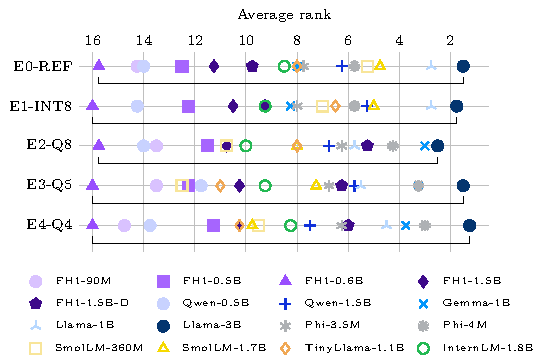
\includegraphics[width=1\linewidth]{Figures/fig4_4_true2d_edge_sequence_nq_open.pdf}
    \caption{NQ-Open token-overlap F1 along the edge-deployment sequence,
    shown separately from the overall correctness summary.}
    \label{fig:app-nq-edge-sequence}
\end{figure}

\begin{figure}
    \centering
    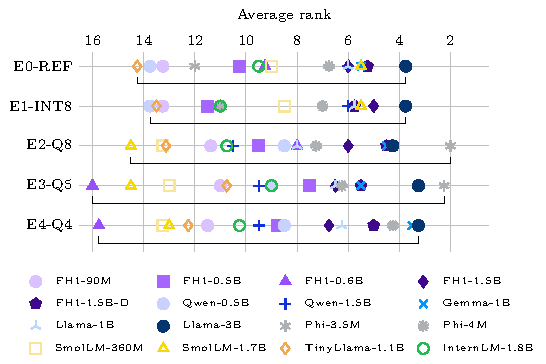
\includegraphics[width=1\linewidth]{Figures/fig4_4_true2d_edge_sequence_squad_v2.pdf}
    \caption{SQuAD v2 token-overlap F1 along the edge-deployment sequence.}
    \label{fig:app-squad-edge-sequence}
\end{figure}


\begin{figure}
    \centering
    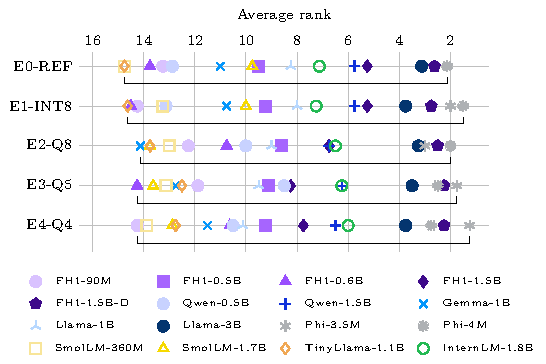
\includegraphics[width=1\linewidth]{Figures/fig4_4_true2d_edge_sequence_truthfulqa_mc1.pdf}
    \caption{TruthfulQA-MC1 accuracy along the edge-deployment sequence.}
    \label{fig:app-truthfulqa-edge-sequence}
\end{figure}



\begin{figure}
    \centering
    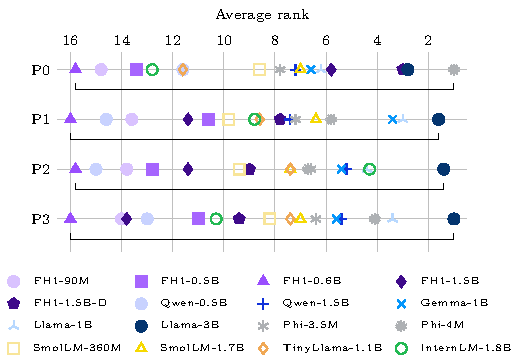
\includegraphics[width=\linewidth]{Figures/fig4_4_true2d_prompt_sequence_nq_open}
    \caption{NQ-Open token-overlap F1 along the prompt-quality sequence.}
    \label{fig:app-nq-prompt-sequence}
\end{figure}

\begin{figure}
    \centering
    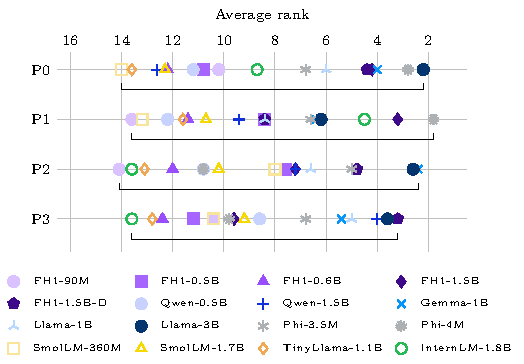
\includegraphics[width=\linewidth]{Figures/fig4_4_true2d_prompt_sequence_squad_v2.pdf}
    \caption{SQuAD v2 token-overlap F1 along the prompt-quality sequence.}
    \label{fig:app-squad-prompt-sequence}
\end{figure}


\begin{figure}
    \centering
    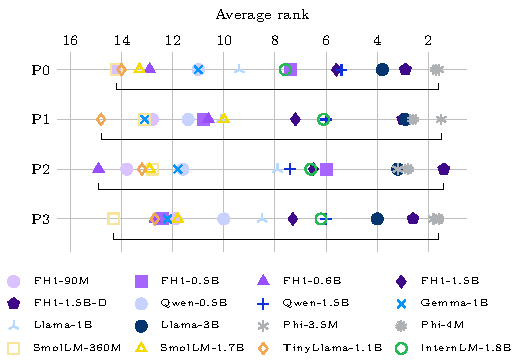
\includegraphics[width=\linewidth]{Figures/fig4_4_true2d_prompt_sequence_truthfulqa_mc1.pdf}
    \caption{TruthfulQA-MC1 accuracy along the prompt-quality sequence.}
    \label{fig:app-truthfulqa-prompt-sequence}
\end{figure}

\begin{table*}[t]
\centering
\scriptsize
\setlength{\tabcolsep}{2.2pt}
\renewcommand{\arraystretch}{0.92}
\caption{NQ-Open token-overlap F1 (\%) across edge settings and prompt tiers. Cell color is normalized within each edge-setting block; greener cells indicate higher F1. Strict exact match is near zero (see Table~\ref{tab:short-answer-true-em}).}
\label{tab:nq-open-correctness-grid}
\resizebox{\textwidth}{!}{%
\begin{tabular}{rrrrr|rrrr|rrrr|rrrr|rrrr}
\toprule
\multirow{2}{*}{Model} & \multicolumn{4}{c}{E0-REF} & \multicolumn{4}{c}{E1-INT8} & \multicolumn{4}{c}{E2-Q8} & \multicolumn{4}{c}{E3-Q5} & \multicolumn{4}{c}{E4-Q4} \\
\cmidrule(lr){2-5} \cmidrule(lr){6-9} \cmidrule(lr){10-13} \cmidrule(lr){14-17} \cmidrule(lr){18-21}
 & P0 & P1 & P2 & P3 & P0 & P1 & P2 & P3 & P0 & P1 & P2 & P3 & P0 & P1 & P2 & P3 & P0 & P1 & P2 & P3 \\
\midrule
FH1-90M & \cellcolor[HTML]{F9D0CC}1.9 & \cellcolor[HTML]{F9CFCC}1.8 & \cellcolor[HTML]{F8CECC}1.5 & \cellcolor[HTML]{F8CDCC}1.2 & \cellcolor[HTML]{F9D0CC}1.9 & \cellcolor[HTML]{F8CECC}1.5 & \cellcolor[HTML]{F8CECC}1.5 & \cellcolor[HTML]{F8CDCC}1.2 & \cellcolor[HTML]{F9D2CC}1.4 & \cellcolor[HTML]{F9D2CC}1.4 & \cellcolor[HTML]{F9D0CC}1.2 & \cellcolor[HTML]{F9D0CC}1.2 & \cellcolor[HTML]{F9D1CC}1.0 & \cellcolor[HTML]{FAD4CC}1.4 & \cellcolor[HTML]{F9D3CC}1.2 & \cellcolor[HTML]{F9D2CC}1.1 & \cellcolor[HTML]{F8CCCC}0.4 & \cellcolor[HTML]{F9D1CC}1.0 & \cellcolor[HTML]{F9D2CC}1.1 & \cellcolor[HTML]{F8CECC}0.6 \\
FH1-0.5B & \cellcolor[HTML]{FBDCCC}4.5 & \cellcolor[HTML]{F9CFCC}1.7 & \cellcolor[HTML]{F9D0CC}1.8 & \cellcolor[HTML]{F9D2CC}2.3 & \cellcolor[HTML]{FBDCCC}4.7 & \cellcolor[HTML]{F9CFCC}1.7 & \cellcolor[HTML]{F9CFCC}1.7 & \cellcolor[HTML]{F9D1CC}2.1 & \cellcolor[HTML]{F9D0CC}1.1 & \cellcolor[HTML]{FAD5CC}1.7 & \cellcolor[HTML]{FAD4CC}1.6 & \cellcolor[HTML]{F9D2CC}1.4 & \cellcolor[HTML]{F9D4CC}1.3 & \cellcolor[HTML]{FAD6CC}1.7 & \cellcolor[HTML]{F9D1CC}0.9 & \cellcolor[HTML]{F9D4CC}1.3 & \cellcolor[HTML]{FAD5CC}1.5 & \cellcolor[HTML]{FAD6CC}1.6 & \cellcolor[HTML]{F9D2CC}1.1 & \cellcolor[HTML]{F9D3CC}1.3 \\
FH1-0.6B & \cellcolor[HTML]{F8CCCC}1.1 & \cellcolor[HTML]{F8CDCC}1.2 & \cellcolor[HTML]{F8CDCC}1.2 & \cellcolor[HTML]{F8CCCC}1.0 & \cellcolor[HTML]{F8CCCC}1.1 & \cellcolor[HTML]{F8CCCC}1.0 & \cellcolor[HTML]{F8CDCC}1.2 & \cellcolor[HTML]{F8CCCC}1.1 & \cellcolor[HTML]{F9D0CC}1.2 & \cellcolor[HTML]{F9CFCC}1.0 & \cellcolor[HTML]{F8CCCC}0.7 & \cellcolor[HTML]{F8CDCC}0.8 & \cellcolor[HTML]{F8CECC}0.5 & \cellcolor[HTML]{F8CECC}0.5 & \cellcolor[HTML]{F8CECC}0.5 & \cellcolor[HTML]{F8CCCC}0.2 & \cellcolor[HTML]{F8CCCC}0.4 & \cellcolor[HTML]{F8CDCC}0.5 & \cellcolor[HTML]{F8CCCC}0.4 & \cellcolor[HTML]{F8CCCC}0.4 \\
FH1-1.5B & \cellcolor[HTML]{FDE9CC}7.4 & \cellcolor[HTML]{F9D2CC}2.3 & \cellcolor[HTML]{F9D0CC}1.9 & \cellcolor[HTML]{F9D1CC}2.0 & \cellcolor[HTML]{FEEFCC}8.8 & \cellcolor[HTML]{F9D1CC}2.2 & \cellcolor[HTML]{F9D0CC}1.8 & \cellcolor[HTML]{F9D0CC}2.0 & \cellcolor[HTML]{FDF2CC}5.2 & \cellcolor[HTML]{F9D3CC}1.4 & \cellcolor[HTML]{F9D3CC}1.5 & \cellcolor[HTML]{F8CDCC}0.8 & \cellcolor[HTML]{FCE2CC}3.4 & \cellcolor[HTML]{FAD5CC}1.5 & \cellcolor[HTML]{FAD5CC}1.5 & \cellcolor[HTML]{F9D2CC}1.0 & \cellcolor[HTML]{FDE8CC}3.9 & \cellcolor[HTML]{F9D3CC}1.3 & \cellcolor[HTML]{FAD5CC}1.4 & \cellcolor[HTML]{F9CFCC}0.7 \\
FH1-1.5B-D & \cellcolor[HTML]{EFEFCC}12.0 & \cellcolor[HTML]{F9D1CC}2.1 & \cellcolor[HTML]{F9D1CC}2.2 & \cellcolor[HTML]{F9D1CC}2.1 & \cellcolor[HTML]{EAEECC}13.1 & \cellcolor[HTML]{F9D0CC}2.0 & \cellcolor[HTML]{F9D1CC}2.1 & \cellcolor[HTML]{F9D1CC}2.1 & \cellcolor[HTML]{DDEBCC}7.9 & \cellcolor[HTML]{FBDECC}2.7 & \cellcolor[HTML]{FAD7CC}1.9 & \cellcolor[HTML]{F9D3CC}1.5 & \cellcolor[HTML]{FEF2CC}5.6 & \cellcolor[HTML]{FAD8CC}2.0 & \cellcolor[HTML]{FAD8CC}1.9 & \cellcolor[HTML]{FAD6CC}1.6 & \cellcolor[HTML]{F3F0CC}6.1 & \cellcolor[HTML]{FAD7CC}1.8 & \cellcolor[HTML]{FAD8CC}1.9 & \cellcolor[HTML]{FAD5CC}1.5 \\
Qwen-0.5B & \cellcolor[HTML]{FCE0CC}5.3 & \cellcolor[HTML]{F8CDCC}1.2 & \cellcolor[HTML]{F8CDCC}1.2 & \cellcolor[HTML]{F8CDCC}1.3 & \cellcolor[HTML]{FBDCCC}4.6 & \cellcolor[HTML]{F8CDCC}1.3 & \cellcolor[HTML]{F8CDCC}1.2 & \cellcolor[HTML]{F8CDCC}1.2 & \cellcolor[HTML]{FAD7CC}2.0 & \cellcolor[HTML]{F9CFCC}1.1 & \cellcolor[HTML]{F8CECC}1.0 & \cellcolor[HTML]{F9D0CC}1.1 & \cellcolor[HTML]{FBDDCC}2.6 & \cellcolor[HTML]{F9D3CC}1.2 & \cellcolor[HTML]{F9D2CC}1.0 & \cellcolor[HTML]{FAD5CC}1.4 & \cellcolor[HTML]{FAD5CC}1.6 & \cellcolor[HTML]{F9D2CC}1.1 & \cellcolor[HTML]{F9D1CC}1.0 & \cellcolor[HTML]{F9D1CC}1.0 \\
Qwen-1.5B & \cellcolor[HTML]{FEEFCC}8.7 & \cellcolor[HTML]{FAD7CC}3.5 & \cellcolor[HTML]{FAD5CC}3.0 & \cellcolor[HTML]{FADACC}4.0 & \cellcolor[HTML]{FEECCC}8.2 & \cellcolor[HTML]{FAD8CC}3.7 & \cellcolor[HTML]{FAD5CC}3.1 & \cellcolor[HTML]{FAD8CC}3.7 & \cellcolor[HTML]{FCDFCC}2.9 & \cellcolor[HTML]{F9D4CC}1.6 & \cellcolor[HTML]{FCE1CC}3.0 & \cellcolor[HTML]{FAD7CC}1.9 & \cellcolor[HTML]{FCE4CC}3.6 & \cellcolor[HTML]{FAD7CC}1.7 & \cellcolor[HTML]{FBDDCC}2.5 & \cellcolor[HTML]{FAD7CC}1.8 & \cellcolor[HTML]{FBDECC}2.6 & \cellcolor[HTML]{FAD8CC}1.8 & \cellcolor[HTML]{FAD5CC}1.6 & \cellcolor[HTML]{FAD6CC}1.7 \\
Gemma-1B & \cellcolor[HTML]{FDEACC}7.5 & \cellcolor[HTML]{FAD8CC}3.7 & \cellcolor[HTML]{F9D3CC}2.6 & \cellcolor[HTML]{F9D4CC}2.8 & \cellcolor[HTML]{FDE7CC}7.0 & \cellcolor[HTML]{FAD7CC}3.5 & \cellcolor[HTML]{F9D3CC}2.7 & \cellcolor[HTML]{F9D4CC}2.8 & \cellcolor[HTML]{FDE6CC}3.6 & \cellcolor[HTML]{FCE0CC}2.9 & \cellcolor[HTML]{FCE1CC}3.0 & \cellcolor[HTML]{FBDDCC}2.6 & \cellcolor[HTML]{FDE8CC}4.2 & \cellcolor[HTML]{FBDFCC}2.8 & \cellcolor[HTML]{FBDBCC}2.4 & \cellcolor[HTML]{FBDCCC}2.5 & \cellcolor[HTML]{FCE3CC}3.3 & \cellcolor[HTML]{FBDCCC}2.4 & \cellcolor[HTML]{FBDACC}2.2 & \cellcolor[HTML]{FCDFCC}2.8 \\
Llama-1B & \cellcolor[HTML]{FDF2CC}9.6 & \cellcolor[HTML]{FCE3CC}6.1 & \cellcolor[HTML]{FCE2CC}5.9 & \cellcolor[HTML]{FCE2CC}5.8 & \cellcolor[HTML]{FBF1CC}10.3 & \cellcolor[HTML]{FCE1CC}5.7 & \cellcolor[HTML]{FCE3CC}6.2 & \cellcolor[HTML]{FCE1CC}5.7 & \cellcolor[HTML]{FCE1CC}3.1 & \cellcolor[HTML]{FAD9CC}2.2 & \cellcolor[HTML]{FAD8CC}2.0 & \cellcolor[HTML]{FAD7CC}1.9 & \cellcolor[HTML]{FCE0CC}3.0 & \cellcolor[HTML]{FBDECC}2.7 & \cellcolor[HTML]{FAD8CC}2.0 & \cellcolor[HTML]{FBDCCC}2.5 & \cellcolor[HTML]{FCE4CC}3.4 & \cellcolor[HTML]{FBDDCC}2.5 & \cellcolor[HTML]{FBDACC}2.1 & \cellcolor[HTML]{FBDBCC}2.2 \\
Llama-3B & \cellcolor[HTML]{EDEECC}12.3 & \cellcolor[HTML]{FDE9CC}7.4 & \cellcolor[HTML]{FDE6CC}6.8 & \cellcolor[HTML]{FCE4CC}6.3 & \cellcolor[HTML]{EFEFCC}12.3 & \cellcolor[HTML]{FDE6CC}6.8 & \cellcolor[HTML]{FDE4CC}6.5 & \cellcolor[HTML]{FCE2CC}6.0 & \cellcolor[HTML]{E3ECCC}7.4 & \cellcolor[HTML]{FBDDCC}2.6 & \cellcolor[HTML]{FBDDCC}2.7 & \cellcolor[HTML]{FCE2CC}3.2 & \cellcolor[HTML]{E0ECCC}8.7 & \cellcolor[HTML]{FBDECC}2.8 & \cellcolor[HTML]{FBDFCC}2.8 & \cellcolor[HTML]{FCE4CC}3.5 & \cellcolor[HTML]{E9EECC}7.1 & \cellcolor[HTML]{FCE3CC}3.3 & \cellcolor[HTML]{FCE0CC}2.8 & \cellcolor[HTML]{FCE4CC}3.3 \\
Phi-3.5M & \cellcolor[HTML]{CEE8CC}17.4 & \cellcolor[HTML]{F9D4CC}2.7 & \cellcolor[HTML]{F9D3CC}2.6 & \cellcolor[HTML]{FAD4CC}2.9 & \cellcolor[HTML]{CEE8CC}17.9 & \cellcolor[HTML]{FAD4CC}2.9 & \cellcolor[HTML]{F9D3CC}2.5 & \cellcolor[HTML]{F9D4CC}2.7 & \cellcolor[HTML]{FAD8CC}2.1 & \cellcolor[HTML]{FAD9CC}2.1 & \cellcolor[HTML]{FBDACC}2.2 & \cellcolor[HTML]{FBDACC}2.2 & \cellcolor[HTML]{FAD7CC}1.8 & \cellcolor[HTML]{FBDACC}2.2 & \cellcolor[HTML]{FBDBCC}2.3 & \cellcolor[HTML]{FBDBCC}2.3 & \cellcolor[HTML]{FAD7CC}1.7 & \cellcolor[HTML]{FBDACC}2.1 & \cellcolor[HTML]{FBDACC}2.1 & \cellcolor[HTML]{FBDCCC}2.3 \\
Phi-4M & \cellcolor[HTML]{CCE8CC}17.7 & \cellcolor[HTML]{FAD6CC}3.3 & \cellcolor[HTML]{FAD6CC}3.1 & \cellcolor[HTML]{FAD7CC}3.4 & \cellcolor[HTML]{CCE8CC}18.2 & \cellcolor[HTML]{FAD6CC}3.2 & \cellcolor[HTML]{F9D4CC}2.8 & \cellcolor[HTML]{FAD6CC}3.3 & \cellcolor[HTML]{CCE8CC}9.3 & \cellcolor[HTML]{FAD9CC}2.1 & \cellcolor[HTML]{FAD7CC}2.0 & \cellcolor[HTML]{FCE1CC}3.1 & \cellcolor[HTML]{CCE8CC}10.9 & \cellcolor[HTML]{FBDBCC}2.3 & \cellcolor[HTML]{FAD8CC}2.0 & \cellcolor[HTML]{FBDFCC}2.8 & \cellcolor[HTML]{CCE8CC}9.8 & \cellcolor[HTML]{FBDECC}2.6 & \cellcolor[HTML]{FAD8CC}1.9 & \cellcolor[HTML]{FBDECC}2.6 \\
SmolLM-360M & \cellcolor[HTML]{FCE1CC}5.6 & \cellcolor[HTML]{FAD9CC}3.9 & \cellcolor[HTML]{FAD9CC}3.8 & \cellcolor[HTML]{FBDBCC}4.3 & \cellcolor[HTML]{FCE3CC}6.2 & \cellcolor[HTML]{FAD8CC}3.7 & \cellcolor[HTML]{FAD5CC}3.0 & \cellcolor[HTML]{FAD6CC}3.3 & \cellcolor[HTML]{FCE0CC}2.9 & \cellcolor[HTML]{F9D1CC}1.2 & \cellcolor[HTML]{F9D1CC}1.3 & \cellcolor[HTML]{F9D4CC}1.5 & \cellcolor[HTML]{FCE1CC}3.1 & \cellcolor[HTML]{F9D3CC}1.2 & \cellcolor[HTML]{F9D3CC}1.2 & \cellcolor[HTML]{F9D2CC}1.0 & \cellcolor[HTML]{FCE3CC}3.2 & \cellcolor[HTML]{F9D3CC}1.2 & \cellcolor[HTML]{FAD5CC}1.5 & \cellcolor[HTML]{FAD5CC}1.5 \\
SmolLM-1.7B & \cellcolor[HTML]{FEECCC}8.0 & \cellcolor[HTML]{FAD9CC}3.9 & \cellcolor[HTML]{FAD9CC}3.9 & \cellcolor[HTML]{FAD9CC}3.8 & \cellcolor[HTML]{FDE8CC}7.4 & \cellcolor[HTML]{FAD9CC}3.9 & \cellcolor[HTML]{FAD9CC}4.0 & \cellcolor[HTML]{FAD7CC}3.5 & \cellcolor[HTML]{FDE7CC}3.8 & \cellcolor[HTML]{FAD5CC}1.8 & \cellcolor[HTML]{FAD6CC}1.8 & \cellcolor[HTML]{F9D3CC}1.5 & \cellcolor[HTML]{FCE2CC}3.3 & \cellcolor[HTML]{FAD8CC}1.9 & \cellcolor[HTML]{FAD6CC}1.7 & \cellcolor[HTML]{FAD9CC}2.0 & \cellcolor[HTML]{FBDFCC}2.7 & \cellcolor[HTML]{F9D4CC}1.4 & \cellcolor[HTML]{F9D3CC}1.2 & \cellcolor[HTML]{F9D3CC}1.3 \\
TinyLlama-1.1B & \cellcolor[HTML]{FAD9CC}3.8 & \cellcolor[HTML]{FAD6CC}3.1 & \cellcolor[HTML]{FAD9CC}3.9 & \cellcolor[HTML]{FAD8CC}3.7 & \cellcolor[HTML]{FAD9CC}3.9 & \cellcolor[HTML]{FAD6CC}3.3 & \cellcolor[HTML]{FBDACC}4.2 & \cellcolor[HTML]{FAD9CC}3.9 & \cellcolor[HTML]{FBDBCC}2.3 & \cellcolor[HTML]{FBDCCC}2.5 & \cellcolor[HTML]{F9D3CC}1.5 & \cellcolor[HTML]{F9D4CC}1.6 & \cellcolor[HTML]{FAD8CC}1.9 & \cellcolor[HTML]{FAD5CC}1.5 & \cellcolor[HTML]{FAD5CC}1.5 & \cellcolor[HTML]{FAD4CC}1.4 & \cellcolor[HTML]{FAD8CC}1.9 & \cellcolor[HTML]{F9D4CC}1.3 & \cellcolor[HTML]{FAD8CC}1.8 & \cellcolor[HTML]{F9D3CC}1.2 \\
InternLM-1.8B & \cellcolor[HTML]{FAD7CC}3.5 & \cellcolor[HTML]{FAD8CC}3.7 & \cellcolor[HTML]{FAD6CC}3.1 & \cellcolor[HTML]{FAD7CC}3.4 & \cellcolor[HTML]{FAD6CC}3.3 & \cellcolor[HTML]{FAD6CC}3.2 & \cellcolor[HTML]{FAD5CC}3.1 & \cellcolor[HTML]{FAD5CC}3.1 & \cellcolor[HTML]{FAD6CC}1.8 & \cellcolor[HTML]{FAD4CC}1.6 & \cellcolor[HTML]{FAD9CC}2.2 & \cellcolor[HTML]{F9D0CC}1.2 & \cellcolor[HTML]{FAD6CC}1.7 & \cellcolor[HTML]{FAD5CC}1.5 & \cellcolor[HTML]{FBDECC}2.8 & \cellcolor[HTML]{F9D4CC}1.3 & \cellcolor[HTML]{FBDDCC}2.5 & \cellcolor[HTML]{FAD6CC}1.6 & \cellcolor[HTML]{FBDDCC}2.5 & \cellcolor[HTML]{F9D3CC}1.2 \\
\bottomrule
\end{tabular}%
}
\end{table*}

\begin{table}[t]
\centering
\caption{Strict exact match (\%) for short-answer QA averaged across models,
using the standard SQuAD/NQ exact-match scorer. Unlike the token-overlap F1
reported in the model-level grids, strict EM is near-zero for weak prompts and
low even under expert prompts, indicating that these SLMs rarely emit the exact
gold span.}
\label{tab:short-answer-true-em}
\setlength{\tabcolsep}{2.4pt}
\renewcommand{\arraystretch}{0.92}
\begin{tabular}{rcccc|cccc}
\toprule
Edge & \multicolumn{4}{c}{SQuAD v2} & \multicolumn{4}{c}{NQ-Open} \\
\cmidrule(lr){2-5} \cmidrule(lr){6-9}
 & P0 & P1 & P2 & P3 & P0 & P1 & P2 & P3 \\
\midrule
E0-REF  & 20.8 & 7.9 & 0.1 & 0.0 & 1.6 & 0.0 & 0.0 & 0.0 \\
E1-INT8 & 20.5 & 5.8 & 0.0 & 0.0 & 1.7 & 0.0 & 0.0 & 0.0 \\
E2-Q8   & 22.0 & 12.4 & 0.2 & 0.0 & 0.0 & 0.0 & 0.0 & 0.0 \\
E3-Q5   & 21.8 & 10.9 & 0.1 & 0.0 & 0.0 & 0.0 & 0.0 & 0.0 \\
E4-Q4   & 20.1 & 10.4 & 0.1 & 0.0 & 0.0 & 0.0 & 0.0 & 0.0 \\
\bottomrule
\end{tabular}
\end{table}



\begin{table*}[t]
\centering
\scriptsize
\setlength{\tabcolsep}{2.2pt}
\renewcommand{\arraystretch}{0.92}
\caption{SQuAD v2 token-overlap F1 (\%) across edge settings and prompt tiers. Cell color is normalized within each edge-setting block; greener cells indicate higher F1. Strict exact match is substantially lower (see Table~\ref{tab:short-answer-true-em}).}
\label{tab:squad-v2-correctness-grid}
\resizebox{\textwidth}{!}{%
\begin{tabular}{rrrrr|rrrr|rrrr|rrrr|rrrr}
\toprule
\multirow{2}{*}{Model} & \multicolumn{4}{c}{E0-REF} & \multicolumn{4}{c}{E1-INT8} & \multicolumn{4}{c}{E2-Q8} & \multicolumn{4}{c}{E3-Q5} & \multicolumn{4}{c}{E4-Q4} \\
\cmidrule(lr){2-5} \cmidrule(lr){6-9} \cmidrule(lr){10-13} \cmidrule(lr){14-17} \cmidrule(lr){18-21}
 & P0 & P1 & P2 & P3 & P0 & P1 & P2 & P3 & P0 & P1 & P2 & P3 & P0 & P1 & P2 & P3 & P0 & P1 & P2 & P3 \\
\midrule
FH1-90M & \cellcolor[HTML]{FFF1CC}31.5 & \cellcolor[HTML]{FAD9CC}13.0 & \cellcolor[HTML]{F8CECC}4.5 & \cellcolor[HTML]{F8CCCC}2.9 & \cellcolor[HTML]{FEEDCC}26.8 & \cellcolor[HTML]{FAD8CC}11.5 & \cellcolor[HTML]{F8CFCC}4.3 & \cellcolor[HTML]{F8CDCC}3.2 & \cellcolor[HTML]{FBF1CC}27.3 & \cellcolor[HTML]{FBDBCC}10.1 & \cellcolor[HTML]{F9CFCC}2.1 & \cellcolor[HTML]{F9CFCC}2.3 & \cellcolor[HTML]{FEF2CC}25.5 & \cellcolor[HTML]{FAD8CC}8.6 & \cellcolor[HTML]{F8CDCC}1.4 & \cellcolor[HTML]{F8CECC}2.2 & \cellcolor[HTML]{FCE3CC}15.5 & \cellcolor[HTML]{F9D2CC}4.2 & \cellcolor[HTML]{F8CDCC}1.5 & \cellcolor[HTML]{F9CFCC}2.4 \\
FH1-0.5B & \cellcolor[HTML]{FBDACC}13.6 & \cellcolor[HTML]{FBDDCC}15.9 & \cellcolor[HTML]{F9CFCC}5.4 & \cellcolor[HTML]{F9CFCC}5.1 & \cellcolor[HTML]{FBDCCC}14.4 & \cellcolor[HTML]{FBDFCC}16.4 & \cellcolor[HTML]{F9CFCC}5.0 & \cellcolor[HTML]{F9CFCC}4.7 & \cellcolor[HTML]{E7EDCC}37.1 & \cellcolor[HTML]{FBF1CC}27.2 & \cellcolor[HTML]{F9CFCC}2.5 & \cellcolor[HTML]{F8CFCC}2.0 & \cellcolor[HTML]{D7EACC}43.9 & \cellcolor[HTML]{FEF2CC}25.5 & \cellcolor[HTML]{F9CFCC}3.0 & \cellcolor[HTML]{F8CDCC}2.0 & \cellcolor[HTML]{EDEFCC}33.8 & \cellcolor[HTML]{FFF1CC}24.8 & \cellcolor[HTML]{F9D0CC}3.2 & \cellcolor[HTML]{F8CECC}1.7 \\
FH1-0.6B & \cellcolor[HTML]{F2EFCC}39.1 & \cellcolor[HTML]{FCE1CC}19.1 & \cellcolor[HTML]{F9CFCC}5.3 & \cellcolor[HTML]{F8CECC}4.2 & \cellcolor[HTML]{F6F0CC}35.8 & \cellcolor[HTML]{FCE2CC}18.6 & \cellcolor[HTML]{F8CECC}4.2 & \cellcolor[HTML]{F8CECC}4.1 & \cellcolor[HTML]{FDEACC}19.8 & \cellcolor[HTML]{FCE3CC}15.5 & \cellcolor[HTML]{F9D1CC}3.5 & \cellcolor[HTML]{F9D0CC}3.0 & \cellcolor[HTML]{F8CCCC}1.3 & \cellcolor[HTML]{F8CCCC}1.1 & \cellcolor[HTML]{F8CCCC}1.4 & \cellcolor[HTML]{F8CCCC}1.3 & \cellcolor[HTML]{F8CDCC}1.1 & \cellcolor[HTML]{F8CDCC}0.9 & \cellcolor[HTML]{F8CDCC}0.9 & \cellcolor[HTML]{F8CDCC}1.1 \\
FH1-1.5B & \cellcolor[HTML]{E0ECCC}49.7 & \cellcolor[HTML]{FDE7CC}23.8 & \cellcolor[HTML]{F9CFCC}5.2 & \cellcolor[HTML]{F9CFCC}5.1 & \cellcolor[HTML]{DCEBCC}50.5 & \cellcolor[HTML]{FDE9CC}24.3 & \cellcolor[HTML]{F9D0CC}5.2 & \cellcolor[HTML]{F9CFCC}5.0 & \cellcolor[HTML]{DDEBCC}41.8 & \cellcolor[HTML]{E9EECC}35.9 & \cellcolor[HTML]{F9D0CC}2.9 & \cellcolor[HTML]{F8CFCC}2.1 & \cellcolor[HTML]{DAEBCC}42.7 & \cellcolor[HTML]{EBEECC}34.6 & \cellcolor[HTML]{F9D0CC}3.4 & \cellcolor[HTML]{F8CECC}2.0 & \cellcolor[HTML]{DEECCC}41.2 & \cellcolor[HTML]{F0EFCC}32.4 & \cellcolor[HTML]{F9CFCC}2.7 & \cellcolor[HTML]{F8CFCC}2.2 \\
FH1-1.5B-D & \cellcolor[HTML]{CCE8CC}60.9 & \cellcolor[HTML]{FCE0CC}17.8 & \cellcolor[HTML]{F9CFCC}5.5 & \cellcolor[HTML]{F9CFCC}5.2 & \cellcolor[HTML]{CCE8CC}59.2 & \cellcolor[HTML]{FCE3CC}19.5 & \cellcolor[HTML]{F9CFCC}5.0 & \cellcolor[HTML]{F9CFCC}5.0 & \cellcolor[HTML]{E0ECCC}40.5 & \cellcolor[HTML]{FFF0CC}23.7 & \cellcolor[HTML]{F9D4CC}5.5 & \cellcolor[HTML]{F9D1CC}3.7 & \cellcolor[HTML]{DEECCC}40.5 & \cellcolor[HTML]{FDE8CC}18.5 & \cellcolor[HTML]{F9D0CC}3.5 & \cellcolor[HTML]{F9CFCC}3.0 & \cellcolor[HTML]{E6EDCC}37.4 & \cellcolor[HTML]{FDE6CC}17.4 & \cellcolor[HTML]{F9D2CC}4.1 & \cellcolor[HTML]{F9D0CC}3.4 \\
Qwen-0.5B & \cellcolor[HTML]{FBDECC}16.4 & \cellcolor[HTML]{FBDBCC}14.6 & \cellcolor[HTML]{F8CECC}4.1 & \cellcolor[HTML]{F8CCCC}3.3 & \cellcolor[HTML]{FCDFCC}16.7 & \cellcolor[HTML]{FBDCCC}14.5 & \cellcolor[HTML]{F8CECC}3.9 & \cellcolor[HTML]{F8CECC}3.6 & \cellcolor[HTML]{F7F0CC}29.4 & \cellcolor[HTML]{FCE1CC}14.1 & \cellcolor[HTML]{F9D0CC}2.6 & \cellcolor[HTML]{F9CFCC}2.6 & \cellcolor[HTML]{FEEECC}22.8 & \cellcolor[HTML]{FAD8CC}8.5 & \cellcolor[HTML]{F9CFCC}3.0 & \cellcolor[HTML]{F8CECC}2.4 & \cellcolor[HTML]{ECEECC}34.4 & \cellcolor[HTML]{FBDCCC}11.1 & \cellcolor[HTML]{F9CFCC}2.6 & \cellcolor[HTML]{F9CFCC}2.4 \\
Qwen-1.5B & \cellcolor[HTML]{FCE0CC}18.0 & \cellcolor[HTML]{FCE4CC}20.9 & \cellcolor[HTML]{F9D0CC}5.7 & \cellcolor[HTML]{F9D0CC}6.1 & \cellcolor[HTML]{FCE4CC}20.6 & \cellcolor[HTML]{FDE5CC}20.8 & \cellcolor[HTML]{F9D1CC}6.2 & \cellcolor[HTML]{F9D1CC}6.0 & \cellcolor[HTML]{FDE7CC}17.8 & \cellcolor[HTML]{FBDDCC}11.6 & \cellcolor[HTML]{F9CFCC}2.6 & \cellcolor[HTML]{F9CFCC}2.5 & \cellcolor[HTML]{FCE2CC}14.9 & \cellcolor[HTML]{FCE1CC}14.1 & \cellcolor[HTML]{F8CECC}2.5 & \cellcolor[HTML]{F9CFCC}2.8 & \cellcolor[HTML]{FBDECC}12.4 & \cellcolor[HTML]{FBDECC}11.9 & \cellcolor[HTML]{F9D0CC}2.9 & \cellcolor[HTML]{F8CFCC}2.3 \\
Gemma-1B & \cellcolor[HTML]{EFEFCC}40.8 & \cellcolor[HTML]{FEEBCC}26.4 & \cellcolor[HTML]{F9D3CC}8.4 & \cellcolor[HTML]{F8CFCC}4.9 & \cellcolor[HTML]{F1EFCC}38.7 & \cellcolor[HTML]{FEEDCC}26.9 & \cellcolor[HTML]{FAD4CC}8.5 & \cellcolor[HTML]{F9D0CC}5.3 & \cellcolor[HTML]{D4EACC}46.1 & \cellcolor[HTML]{FDE7CC}17.9 & \cellcolor[HTML]{FAD6CC}6.7 & \cellcolor[HTML]{F9D0CC}3.1 & \cellcolor[HTML]{CEE8CC}48.1 & \cellcolor[HTML]{FCE3CC}15.7 & \cellcolor[HTML]{F9D2CC}5.1 & \cellcolor[HTML]{F8CECC}2.1 & \cellcolor[HTML]{CCE8CC}49.9 & \cellcolor[HTML]{FEECCC}21.2 & \cellcolor[HTML]{FAD4CC}5.9 & \cellcolor[HTML]{F9D0CC}3.3 \\
Llama-1B & \cellcolor[HTML]{EBEECC}43.3 & \cellcolor[HTML]{FBDBCC}14.4 & \cellcolor[HTML]{F9D4CC}8.8 & \cellcolor[HTML]{F9CFCC}5.4 & \cellcolor[HTML]{EAEECC}42.8 & \cellcolor[HTML]{FBDBCC}14.0 & \cellcolor[HTML]{FAD5CC}9.1 & \cellcolor[HTML]{F9D0CC}5.5 & \cellcolor[HTML]{E3EDCC}38.9 & \cellcolor[HTML]{FDF2CC}26.4 & \cellcolor[HTML]{F9CFCC}2.6 & \cellcolor[HTML]{F9CFCC}2.1 & \cellcolor[HTML]{D8EACC}43.3 & \cellcolor[HTML]{F7F0CC}28.9 & \cellcolor[HTML]{F8CECC}2.6 & \cellcolor[HTML]{F8CECC}2.2 & \cellcolor[HTML]{E6EDCC}37.3 & \cellcolor[HTML]{FEF2CC}25.6 & \cellcolor[HTML]{F9CFCC}2.5 & \cellcolor[HTML]{F9CFCC}2.6 \\
Llama-3B & \cellcolor[HTML]{E6EDCC}46.4 & \cellcolor[HTML]{FCDFCC}17.5 & \cellcolor[HTML]{FAD7CC}11.5 & \cellcolor[HTML]{F9D3CC}8.1 & \cellcolor[HTML]{E5EDCC}45.5 & \cellcolor[HTML]{FCE0CC}17.7 & \cellcolor[HTML]{FAD7CC}10.4 & \cellcolor[HTML]{F9D3CC}7.7 & \cellcolor[HTML]{CCE8CC}50.2 & \cellcolor[HTML]{F5F0CC}30.1 & \cellcolor[HTML]{F9D1CC}3.6 & \cellcolor[HTML]{F9CFCC}2.2 & \cellcolor[HTML]{CCE8CC}49.2 & \cellcolor[HTML]{F8F1CC}28.6 & \cellcolor[HTML]{F9D2CC}4.6 & \cellcolor[HTML]{F8CFCC}2.7 & \cellcolor[HTML]{CCE8CC}50.0 & \cellcolor[HTML]{FEF2CC}25.6 & \cellcolor[HTML]{F9D1CC}3.7 & \cellcolor[HTML]{F9CFCC}2.6 \\
Phi-3.5M & \cellcolor[HTML]{FCE0CC}18.0 & \cellcolor[HTML]{FAD7CC}11.5 & \cellcolor[HTML]{F8CECC}4.7 & \cellcolor[HTML]{F8CFCC}4.8 & \cellcolor[HTML]{FDE8CC}23.1 & \cellcolor[HTML]{FAD9CC}12.4 & \cellcolor[HTML]{F9CFCC}4.9 & \cellcolor[HTML]{F9CFCC}4.9 & \cellcolor[HTML]{D9EBCC}43.7 & \cellcolor[HTML]{E4EDCC}38.5 & \cellcolor[HTML]{FAD7CC}7.7 & \cellcolor[HTML]{F9D0CC}3.2 & \cellcolor[HTML]{D5EACC}44.9 & \cellcolor[HTML]{E1ECCC}39.4 & \cellcolor[HTML]{FAD5CC}6.8 & \cellcolor[HTML]{F8CFCC}2.8 & \cellcolor[HTML]{DAEBCC}43.4 & \cellcolor[HTML]{E5EDCC}37.9 & \cellcolor[HTML]{FAD7CC}7.8 & \cellcolor[HTML]{F8CFCC}2.2 \\
Phi-4M & \cellcolor[HTML]{E4EDCC}47.0 & \cellcolor[HTML]{FEEDCC}28.0 & \cellcolor[HTML]{F8CECC}4.8 & \cellcolor[HTML]{F8CECC}4.4 & \cellcolor[HTML]{E3ECCC}46.7 & \cellcolor[HTML]{FEEBCC}25.4 & \cellcolor[HTML]{F9CFCC}4.8 & \cellcolor[HTML]{F8CFCC}4.4 & \cellcolor[HTML]{D3E9CC}46.6 & \cellcolor[HTML]{E4EDCC}38.4 & \cellcolor[HTML]{F9CFCC}2.1 & \cellcolor[HTML]{F8CFCC}2.1 & \cellcolor[HTML]{D4E9CC}45.6 & \cellcolor[HTML]{E1ECCC}39.4 & \cellcolor[HTML]{F8CECC}2.5 & \cellcolor[HTML]{F8CECC}2.1 & \cellcolor[HTML]{D3E9CC}46.4 & \cellcolor[HTML]{E2ECCC}39.3 & \cellcolor[HTML]{F9D0CC}2.9 & \cellcolor[HTML]{F9CFCC}2.4 \\
SmolLM-360M & \cellcolor[HTML]{FCDFCC}17.7 & \cellcolor[HTML]{FCDFCC}17.5 & \cellcolor[HTML]{F9CFCC}5.4 & \cellcolor[HTML]{F9CFCC}5.3 & \cellcolor[HTML]{FCE0CC}17.1 & \cellcolor[HTML]{FCE0CC}17.1 & \cellcolor[HTML]{F9D1CC}6.1 & \cellcolor[HTML]{F9CFCC}5.0 & \cellcolor[HTML]{FAD8CC}8.3 & \cellcolor[HTML]{F8CCCC}0.3 & \cellcolor[HTML]{F9D0CC}2.8 & \cellcolor[HTML]{F8CECC}1.9 & \cellcolor[HTML]{FBDBCC}10.4 & \cellcolor[HTML]{FAD6CC}7.2 & \cellcolor[HTML]{F8CFCC}2.7 & \cellcolor[HTML]{F8CDCC}1.4 & \cellcolor[HTML]{FAD5CC}6.5 & \cellcolor[HTML]{F8CCCC}0.5 & \cellcolor[HTML]{F8CECC}2.1 & \cellcolor[HTML]{F8CFCC}2.2 \\
SmolLM-1.7B & \cellcolor[HTML]{F5F0CC}37.4 & \cellcolor[HTML]{FDE7CC}23.7 & \cellcolor[HTML]{F9CFCC}5.5 & \cellcolor[HTML]{F9CFCC}5.5 & \cellcolor[HTML]{F2EFCC}38.0 & \cellcolor[HTML]{FDE6CC}21.6 & \cellcolor[HTML]{F9D0CC}5.7 & \cellcolor[HTML]{F9D0CC}5.4 & \cellcolor[HTML]{FCE1CC}14.3 & \cellcolor[HTML]{F8CDCC}1.2 & \cellcolor[HTML]{F9CFCC}2.4 & \cellcolor[HTML]{F8CECC}1.6 & \cellcolor[HTML]{FAD6CC}7.2 & \cellcolor[HTML]{F9D4CC}6.0 & \cellcolor[HTML]{F8CECC}2.0 & \cellcolor[HTML]{F8CDCC}1.7 & \cellcolor[HTML]{FAD5CC}6.2 & \cellcolor[HTML]{F8CDCC}1.4 & \cellcolor[HTML]{F8CECC}1.8 & \cellcolor[HTML]{F8CFCC}2.3 \\
TinyLlama-1.1B & \cellcolor[HTML]{FBDECC}16.3 & \cellcolor[HTML]{F9D2CC}7.2 & \cellcolor[HTML]{F8CECC}4.4 & \cellcolor[HTML]{F8CECC}4.3 & \cellcolor[HTML]{FBDECC}16.2 & \cellcolor[HTML]{F9D3CC}7.5 & \cellcolor[HTML]{F9CFCC}4.8 & \cellcolor[HTML]{F8CFCC}4.4 & \cellcolor[HTML]{FCE4CC}15.8 & \cellcolor[HTML]{FDE8CC}18.7 & \cellcolor[HTML]{F9CFCC}2.1 & \cellcolor[HTML]{F8CECC}1.7 & \cellcolor[HTML]{FCE2CC}15.3 & \cellcolor[HTML]{FDEACC}19.8 & \cellcolor[HTML]{F8CECC}2.1 & \cellcolor[HTML]{F8CECC}2.0 & \cellcolor[HTML]{FCE2CC}14.8 & \cellcolor[HTML]{FEEBCC}21.0 & \cellcolor[HTML]{F8CECC}1.9 & \cellcolor[HTML]{F8CECC}1.6 \\
InternLM-1.8B & \cellcolor[HTML]{EFEFCC}41.1 & \cellcolor[HTML]{F6F0CC}37.1 & \cellcolor[HTML]{F8CCCC}3.1 & \cellcolor[HTML]{F8CCCC}3.3 & \cellcolor[HTML]{F2EFCC}38.0 & \cellcolor[HTML]{FDE6CC}21.6 & \cellcolor[HTML]{F8CCCC}2.5 & \cellcolor[HTML]{F8CCCC}2.4 & \cellcolor[HTML]{FFF2CC}25.0 & \cellcolor[HTML]{FAF1CC}27.5 & \cellcolor[HTML]{F8CECC}1.9 & \cellcolor[HTML]{F8CFCC}2.1 & \cellcolor[HTML]{FCF2CC}26.3 & \cellcolor[HTML]{FBF1CC}26.9 & \cellcolor[HTML]{F8CFCC}2.8 & \cellcolor[HTML]{F8CDCC}1.9 & \cellcolor[HTML]{FEECCC}21.1 & \cellcolor[HTML]{FFF2CC}25.4 & \cellcolor[HTML]{F8CECC}2.0 & \cellcolor[HTML]{F8CECC}1.8 \\
\bottomrule
\end{tabular}%
}
\end{table*}


Table~\ref{tab:ifeval-model-edge-heatmap} gives the model-level IFEval results. IFEval is evaluated under P0
only; its \texttt{prompt\_acc} column is the official IFEval prompt-level
compliance metric, not a PEEL prompt tier.

\begin{table*}[t]
\centering
\scriptsize
\setlength{\tabcolsep}{2.5pt}
\renewcommand{\arraystretch}{0.92}
\caption{IFEval rule-based instruction-following accuracy (\%) across edge settings under P0. Cell colors are normalized within each metric--edge column across models; greener cells indicate higher compliance.}
\label{tab:ifeval-model-edge-heatmap}
\resizebox{\textwidth}{!}{%
\begin{tabular}{lccccc|ccccc}
\toprule
Model & \multicolumn{5}{c}{Instruction-level accuracy} & \multicolumn{5}{c}{Prompt-level accuracy} \\
\cmidrule(lr){2-6} \cmidrule(lr){7-11}
 & E0-REF & E1-INT8 & E2-Q8 & E3-Q5 & E4-Q4 & E0-REF & E1-INT8 & E2-Q8 & E3-Q5 & E4-Q4 \\
\midrule
Falcon-H1-Tiny-90M & \cellcolor[HTML]{ECEED0}68.8 & \cellcolor[HTML]{F0EFCF}64.5 & \cellcolor[HTML]{EFEFCF}62.5 & \cellcolor[HTML]{EEEECF}61.5 & \cellcolor[HTML]{F4F0CE}58.5 & \cellcolor[HTML]{EDEECF}59.1 & \cellcolor[HTML]{F2EFCE}54.0 & \cellcolor[HTML]{F4F0CE}49.9 & \cellcolor[HTML]{F3EFCE}48.8 & \cellcolor[HTML]{F9F1CD}45.1 \\
Falcon-H1-0.5B & \cellcolor[HTML]{E2ECD1}75.1 & \cellcolor[HTML]{E8EDD0}69.8 & \cellcolor[HTML]{E1ECD2}71.8 & \cellcolor[HTML]{E0EBD2}71.2 & \cellcolor[HTML]{E2ECD1}70.1 & \cellcolor[HTML]{E5ECD1}64.5 & \cellcolor[HTML]{EAEED0}59.1 & \cellcolor[HTML]{E3ECD1}61.2 & \cellcolor[HTML]{E1ECD1}60.1 & \cellcolor[HTML]{E4ECD1}58.8 \\
Falcon-H1-Tiny-R-0.6B & \cellcolor[HTML]{FEEFCC}53.5 & \cellcolor[HTML]{FEEFCC}52.8 & \cellcolor[HTML]{FEEFCC}49.5 & \cellcolor[HTML]{F4CCCC}24.8 & \cellcolor[HTML]{F4CCCC}25.7 & \cellcolor[HTML]{FDEACC}41.0 & \cellcolor[HTML]{FCE9CC}39.5 & \cellcolor[HTML]{FCE9CC}36.8 & \cellcolor[HTML]{F4CCCC}15.7 & \cellcolor[HTML]{F4CCCC}15.9 \\
Falcon-H1-1.5B & \cellcolor[HTML]{DAEAD3}80.2 & \cellcolor[HTML]{DEEBD2}76.2 & \cellcolor[HTML]{DBEBD3}75.4 & \cellcolor[HTML]{DBEAD3}74.5 & \cellcolor[HTML]{DBEAD3}75.0 & \cellcolor[HTML]{DBEAD3}71.2 & \cellcolor[HTML]{DEEBD2}66.9 & \cellcolor[HTML]{DEEBD2}64.9 & \cellcolor[HTML]{DBEAD3}64.3 & \cellcolor[HTML]{DBEAD3}64.9 \\
Falcon-H1-1.5B-Deep & \cellcolor[HTML]{D9EAD3}81.2 & \cellcolor[HTML]{D9EAD3}79.6 & \cellcolor[HTML]{D9EAD3}77.0 & \cellcolor[HTML]{D9EAD3}75.8 & \cellcolor[HTML]{D9EAD3}76.1 & \cellcolor[HTML]{D9EAD3}72.5 & \cellcolor[HTML]{D9EAD3}70.4 & \cellcolor[HTML]{D9EAD3}68.0 & \cellcolor[HTML]{D9EAD3}65.6 & \cellcolor[HTML]{D9EAD3}66.4 \\
Qwen2.5-0.5B & \cellcolor[HTML]{F8DACC}39.5 & \cellcolor[HTML]{F8D9CC}38.5 & \cellcolor[HTML]{FADFCC}38.7 & \cellcolor[HTML]{FBE4CC}40.9 & \cellcolor[HTML]{FBE5CC}42.1 & \cellcolor[HTML]{F8D9CC}29.8 & \cellcolor[HTML]{F8DACC}29.4 & \cellcolor[HTML]{F9DCCC}28.5 & \cellcolor[HTML]{FAE2CC}30.3 & \cellcolor[HTML]{FBE4CC}31.8 \\
Qwen2.5-1.5B & \cellcolor[HTML]{FDECCC}51.8 & \cellcolor[HTML]{FEF0CC}53.5 & \cellcolor[HTML]{FCF1CD}53.7 & \cellcolor[HTML]{FAF1CD}53.6 & \cellcolor[HTML]{FEEDCC}47.7 & \cellcolor[HTML]{FDEACC}41.0 & \cellcolor[HTML]{FEEECC}42.5 & \cellcolor[HTML]{FFF2CC}42.5 & \cellcolor[HTML]{FCF1CD}42.7 & \cellcolor[HTML]{FDEBCC}36.2 \\
Gemma-3-1B & \cellcolor[HTML]{EFEFCF}66.4 & \cellcolor[HTML]{EDEECF}66.3 & \cellcolor[HTML]{F4F0CE}59.0 & \cellcolor[HTML]{F4F0CE}57.4 & \cellcolor[HTML]{F3EFCE}59.1 & \cellcolor[HTML]{F3EFCE}55.1 & \cellcolor[HTML]{F2EFCE}54.2 & \cellcolor[HTML]{F8F0CD}47.7 & \cellcolor[HTML]{F7F0CD}45.7 & \cellcolor[HTML]{F6F0CE}47.3 \\
Llama-3.2-1B & \cellcolor[HTML]{F3EFCE}64.1 & \cellcolor[HTML]{EFEFCF}65.3 & \cellcolor[HTML]{EFEFCF}62.5 & \cellcolor[HTML]{EDEECF}62.5 & \cellcolor[HTML]{EDEECF}62.8 & \cellcolor[HTML]{F6F0CE}52.5 & \cellcolor[HTML]{F3EFCE}53.4 & \cellcolor[HTML]{F2EFCE}51.2 & \cellcolor[HTML]{EFEFCF}51.2 & \cellcolor[HTML]{EFEFCF}51.9 \\
Llama-3.2-3B & \cellcolor[HTML]{E0EBD2}76.7 & \cellcolor[HTML]{DFEBD2}75.6 & \cellcolor[HTML]{E1ECD2}71.7 & \cellcolor[HTML]{DEEBD2}72.3 & \cellcolor[HTML]{E0EBD2}71.7 & \cellcolor[HTML]{E2ECD1}66.2 & \cellcolor[HTML]{E2ECD1}64.7 & \cellcolor[HTML]{E4ECD1}61.0 & \cellcolor[HTML]{DFEBD2}61.5 & \cellcolor[HTML]{E2ECD1}60.6 \\
Phi-3.5-mini & \cellcolor[HTML]{FAF1CD}59.2 & \cellcolor[HTML]{F4F0CE}61.9 & \cellcolor[HTML]{F2EFCE}60.2 & \cellcolor[HTML]{F2EFCE}59.2 & \cellcolor[HTML]{F1EFCF}60.5 & \cellcolor[HTML]{FFF2CC}46.6 & \cellcolor[HTML]{F9F1CD}49.4 & \cellcolor[HTML]{F9F1CD}47.1 & \cellcolor[HTML]{F5F0CE}47.0 & \cellcolor[HTML]{F6F0CE}47.3 \\
Phi-4-mini & \cellcolor[HTML]{E4ECD1}74.0 & \cellcolor[HTML]{E5EDD1}71.8 & \cellcolor[HTML]{E0EBD2}72.4 & \cellcolor[HTML]{DCEBD2}73.9 & \cellcolor[HTML]{DEEBD2}73.0 & \cellcolor[HTML]{E5ECD1}64.5 & \cellcolor[HTML]{E5EDD1}62.5 & \cellcolor[HTML]{E1ECD1}62.5 & \cellcolor[HTML]{DAEAD3}64.7 & \cellcolor[HTML]{DEEBD2}63.2 \\
SmolLM2-360M & \cellcolor[HTML]{FAE2CC}45.3 & \cellcolor[HTML]{FBE3CC}45.1 & \cellcolor[HTML]{FCE9CC}45.2 & \cellcolor[HTML]{FDEBCC}45.8 & \cellcolor[HTML]{FDE9CC}45.2 & \cellcolor[HTML]{FAE0CC}34.6 & \cellcolor[HTML]{FAE0CC}33.6 & \cellcolor[HTML]{FCE6CC}34.9 & \cellcolor[HTML]{FCE9CC}34.8 & \cellcolor[HTML]{FCE9CC}35.1 \\
SmolLM2-1.7B & \cellcolor[HTML]{F9F1CD}59.5 & \cellcolor[HTML]{F8F0CD}59.5 & \cellcolor[HTML]{F6F0CE}57.8 & \cellcolor[HTML]{F2EFCE}59.1 & \cellcolor[HTML]{F4F0CE}58.5 & \cellcolor[HTML]{FFF1CC}46.0 & \cellcolor[HTML]{FDF2CC}47.0 & \cellcolor[HTML]{FBF1CD}45.3 & \cellcolor[HTML]{F5F0CE}47.0 & \cellcolor[HTML]{F8F0CD}46.0 \\
TinyLlama-1.1B & \cellcolor[HTML]{F4CCCC}30.4 & \cellcolor[HTML]{F4CCCC}29.9 & \cellcolor[HTML]{F4CCCC}25.9 & \cellcolor[HTML]{F5D0CC}27.4 & \cellcolor[HTML]{F6D2CC}29.5 & \cellcolor[HTML]{F4CCCC}20.7 & \cellcolor[HTML]{F4CCCC}20.5 & \cellcolor[HTML]{F4CCCC}17.6 & \cellcolor[HTML]{F6D1CC}19.2 & \cellcolor[HTML]{F6D3CC}20.5 \\
InternLM-1.8B & \cellcolor[HTML]{FBE5CC}47.2 & \cellcolor[HTML]{FCE6CC}47.1 & \cellcolor[HTML]{FDEACC}46.2 & \cellcolor[HTML]{FDECCC}46.2 & \cellcolor[HTML]{FCE9CC}44.7 & \cellcolor[HTML]{FBE5CC}37.6 & \cellcolor[HTML]{FBE4CC}36.4 & \cellcolor[HTML]{FCE8CC}35.9 & \cellcolor[HTML]{FDEACC}35.5 & \cellcolor[HTML]{FCE8CC}34.2 \\
\bottomrule
\end{tabular}%
}
\end{table*}

\bibliographystyle{aaai2027}
\bibliography{references}

\end{document}
